\documentclass{sosg-informe}

\graphicspath{{figuras/}{../../geodatos/estudios/santa-cruz/figuras/}{../../geodatos/estudios/san-cristobal/figuras/}{../../geodatos/estudios/la-cascada/figuras/}{../../clima/eventos/2026-10-30_inundacion/}}

\title{Lluvia observada del 30--31 de octubre de 2026\\en Santa Cruz y San Cristóbal (Galápagos),\\climatología de extremos y nivel del mar}
\titulocorto{Lluvia del 30--31-oct, climatología y nivel del mar}
\numero{2026-03}
\estado{Borrador para discusión}
\titulocita{Lluvia observada del 30--31 de octubre de 2026 en Santa Cruz y San Cristóbal (Galápagos), climatología de extremos y nivel del mar}
\relacionados{Issues \issue{3}, \issue{13}, \issue{46}, \issue{56}, \issue{57}, \issue{61}, \issue{62}, \issue{73} y \issue{76} · repositorio mayait/sosgalapagos-datos}
\date{4 de noviembre de 2026}

\begin{document}
\maketitle

\begin{abstract}
El 30 de octubre de 2026 una tormenta convectiva inundó el barrio La Cascada (Puerto Ayora, Santa Cruz), y en la mañana del 31 se desbordaron cañadas en Puerto Baquerizo Moreno (San Cristóbal). Este informe reúne lo que midieron los pluviómetros, lo que estimaron los modelos y cómo se sitúa el evento en la climatología y en el ciclo de la marea. Se consolidaron series de 5~min, horarias y diarias de la red IERSE-WSN, del INAMHI y del GSC-USFQ, siempre con su cobertura. En la parte media de Santa Cruz se midieron al menos 178,8~mm (Los Guayabillos) y 237,6~mm (Santa Rosa) el 30-oct, con 61--66~mm en una hora de reloj y 138--139~mm en 3~h móviles. Son mínimos: las dos estaciones dejaron de transmitir a las 21:22--21:25, en plena lluvia, durante 21,3~h. En la costa, el pluviómetro M0191 midió 135,1~mm más entre las 22:00 y las 03:00. El ECMWF de 9~km situó su máximo unas 9~h tarde, con la mitad de la intensidad horaria y un 7--11\,\% de la lluvia en la ventana en que realmente llovió; los demás modelos quedaron muy por debajo. Para octubre y noviembre el día no tiene precedente en más de 30 años de registros cercanos. En régimen anual es un evento de años a decenas de años, y el periodo de retorno depende mucho del método: con Gumbel por momentos y la serie de Bellavista, 179~mm vuelven cada 8 años con el dato dudoso de marzo de 2008 y cada 94 años sin él. El reanálisis GAR, que es lluvia modelada, acierta el nivel medio de los máximos en Puerto Ayora pero no los días concretos. La marea no agravó el evento: el agua llegó al barrio con la marea bajando, aunque el mar estaba unos 0,5~m por encima de la marea astronómica por El Niño.
\palabrasclave{lluvia extrema; pluviómetro de balancín; cortes de transmisión; modelos numéricos; Gumbel; reanálisis GAR; marea; UTide; El Niño; Galápagos.}
\end{abstract}

\begin{aviso}
Este informe combina \textbf{datos medidos} por terceros con \textbf{estimaciones propias y de modelos}, que no son datos oficiales. Los periodos de retorno son un orden de magnitud y no sirven para diseñar obras. La lluvia de los modelos de pronóstico y del reanálisis GAR es lluvia modelada. El nivel del mar en Puerto Baquerizo Moreno es una estimación, porque allí no hay mareógrafo. El análisis lo preparó un equipo asistido por agentes de inteligencia artificial, sin visitas de campo ni revisión profesional externa, y no expresa una posición institucional de la USFQ. Licencias de los datos usados: IERSE, CC BY-NC-ND 4.0 \citep{ierse2023}; FCD, CC BY-NC-SA \citep{fcd2026}; GSC-USFQ, sin licencia declarada, por lo que sus series solo se describen y no se reproducen \citep[\issue{46};][]{gsc2026}; Open-Meteo, CC BY 4.0 \citep{zippenfenig2023}; GAR, CC BY 4.0 \citep{schmidt2025}; UHSLC y NOAA, dominio público \citep{caldwell2015,huang2021}. Del proyecto DARWIN solo se usaron metadatos públicos (\issue{76}).
\end{aviso}

% =====================================================================
\section{Introducción}

Santa Cruz y San Cristóbal no tienen ríos permanentes. El agua de lluvia baja por quebradas secas y se acumula en barrios construidos sobre depresiones o en la salida de esos cauces al mar. En la tarde y la noche del 30 de octubre de 2026 un núcleo convectivo descargó sobre la parte media de Santa Cruz e inundó La Cascada, en Puerto Ayora. En la mañana del 31 se desbordaron las cañadas Barrio Frío y Divino Niño en Puerto Baquerizo Moreno, según el SitRep n.º~01 de la SNGR.

Los informes técnicos de la serie que modelan esas inundaciones (2026-02, 2026-06 y 2026-07) necesitan la lluvia del evento como dato de entrada. Este informe responde a cuatro preguntas previas:
\begin{enumerate}
  \item ¿Cuánto llovió, dónde y a qué hora, y qué parte de esa lluvia no se midió?
  \item ¿Qué estimaron los modelos meteorológicos que se pueden consultar en abierto?
  \item ¿Fue un récord, y cada cuánto vuelve una lluvia así?
  \item ¿Coincidió la lluvia con una marea alta que dificultara el desagüe al mar?
\end{enumerate}

En todo el texto se distingue lo \textbf{medido} (pluviómetros, mareógrafos), lo \textbf{estimado por modelo} (pronósticos, reanálisis, ajustes estadísticos) y lo \textbf{reportado} por fuentes oficiales o la prensa. Todas las horas son de Galápagos (UTC$-6$).

% =====================================================================
\section{Área de estudio y datos}

\subsection{Lluvia medida}
La tabla~\ref{tab:fuentes} resume las fuentes. Ninguna estación de la red IERSE-WSN está en Puerto Ayora: la más cercana a La Cascada es Los Guayabillos, en la parte media de la cuenca.

\begin{table}[ht]
  \centering\footnotesize
  \caption{Fuentes de lluvia medida usadas en este informe y su estado al 2 de noviembre de 2026.}
  \label{tab:fuentes}
  \begin{tabularx}{\linewidth}{>{\raggedright\arraybackslash}p{2.5cm}>{\raggedright\arraybackslash}X>{\raggedright\arraybackslash}p{2.1cm}>{\raggedright\arraybackslash}p{2.1cm}l}
    \toprule
    Fuente & Estaciones (cota) & Resolución & Periodo & Hora \\
    \midrule
    IERSE-WSN \citep{ierse2023} & Cerro Crocker (${\approx}\,861$~m), Santa Rosa (${\approx}\,416$~m), Los Guayabillos (${\approx}\,178$~m), Militar en Baltra (${\approx}\,14$~m) & ${\approx}\,5$~min & abr-2026 $\to$ & UTC$-6$ \\
    INAMHI \citep{inamhi2026} & M0191 Puerto Ayora (6~m) & 1~h (5~min desde el 1-nov) & 16-oct $\to$ 2-nov & UTC$-5$ \\
    GSC-USFQ \citep{gsc2026} & El Junco, Cerro Alto, El Mirador y Merceditas (San Cristóbal, 100--600~m) & 1~h (historial del INAMHI) & 16-oct $\to$ 2-nov & UTC$-5$ \\
    Estación particular (Tempest) & Punta Estrada, Puerto Ayora (8~m) & 1~min $\to$ 5~min & sep-2026 $\to$ & UTC \\
    FCD \citep{fcd2026} & Puerto Ayora (2~m), lectura manual diaria; Bellavista (223~m) & 1~día & 1965--jun-2026; 1987--2019 & --- \\
    \bottomrule
  \end{tabularx}
  \par\vspace{3pt}\raggedright\footnotesize Cotas de la red IERSE-WSN según el DSM Copernicus GLO-30 (error de ${\pm}\,2$--4~m y sesgo de unos $-2$~m frente al IGM); son orientativas.
\end{table}

\subsection{Climatología de referencia}
\begin{itemize}
  \item \textbf{Series diarias de la FCD:} Puerto Ayora desde 1965 (61 años completos) y Bellavista de 1988 a 2018 (31 años completos). La FCD advierte que los datos publicados de Bellavista fueron \enquote{ajustados} al digitalizarlos, y el episodio de marzo de 2008 (490, 280 y 202~mm en tres días) está por verificar con la serie original (\issue{73}).
  \item \textbf{Reanálisis GAR} (\emph{Galápagos Archipelago Refined analysis}; \citealp{schmidt2025}): WRF 4.3.3 a 2~km forzado con ERA5 \citep{hersbach2020}, 1980--2025, CC BY 4.0. Se usó la lluvia diaria (día UTC, de 18:00 a 18:00 en Galápagos) en 14 puntos de las dos islas. Es \emph{lluvia modelada}.
  \item \textbf{Totales publicados:} \citet{paltan2021}, con estaciones del INAMHI de 1981 a 2017, dan unos 500~mm/año (${\pm}\,185$) en la costa de Santa Cruz y San Cristóbal y 1050--1670~mm/año en la parte alta.
\end{itemize}

\subsection{Modelos meteorológicos}
Se pidió a Open-Meteo \citep{zippenfenig2023} la lluvia horaria del 15-oct al 2-nov-2026 de siete modelos: ECMWF IFS de 9~km, ECMWF IFS de 0,25°, NOAA GFS, DWD ICON, JMA, Météo-France y UKMO. La petición se hizo directamente en hora de Galápagos. Cada valor horario es la lluvia de la hora que \emph{termina} en la marca. Para cada estación se tomó la celda del modelo que la contiene.

\subsection{Nivel del mar}
\begin{itemize}
  \item \textbf{Series horarias del UHSLC} \citep{caldwell2015}: Puerto Ayora (Academy Bay, desde 1978) y Baltra. Se usan para ajustar la marea astronómica.
  \item \textbf{Mareógrafos IOC} \citep{ioc2026} de Puerto Ayora y Baltra, operados por el INOCAR, cada minuto. Se usa el sensor de radar \enquote{ras}, que comparte el cero del UHSLC.
  \item \textbf{Open-Meteo Marine:} nivel del mar modelado, cada hora, en las celdas de Puerto Ayora y de Puerto Baquerizo Moreno. Solo se usa para trasladar la marea de una bahía a otra.
\end{itemize}

\subsection{Datos que no se pudieron usar}
El proyecto DARWIN (Universidad de Marburgo y Universidad del Azuay) tiene estaciones automáticas de 10~min en Santa Cruz y San Cristóbal desde 2022 \citep{darwin_sc,darwin_scb}. Santa Rosa, Cerro Crocker y Militar comparten coordenadas con la red IERSE-WSN, así que podrían contener la lluvia del corte. Pero lo publicado termina entre octubre de 2025 y mayo de 2026, y su acuerdo de uso prohíbe redistribuir las series (\issue{76}). Aquí solo se usan sus metadatos públicos. Su lluvia se mide sobre todo con un sensor de radar, que subestima mucho la garúa: en Cerro Crocker midió 283~mm frente a 1707~mm de un balancín, de abril de 2022 a marzo de 2023 \citep{schmidt2025}.

% =====================================================================
\section{Métodos}

\subsection{Series de 5 minutos, horarias y diarias}\label{sec:series}
Cada registro de IERSE-WSN es la lluvia caída desde el registro anterior, en pasos de 0,2~mm del balancín. Los scripts \texttt{clima/scripts/01\_ierse\_descargar.py} y \texttt{02\_ierse\_consolidar.py} guardan los crudos sin modificar y los agregan por hora y por día. La cobertura de un día es
\begin{equation}
  C_d = 100\,\frac{n_d}{288},
\end{equation}
en porcentaje, donde $n_d$ es el número de registros recibidos y 288 los posibles cada 5~min. Un tramo sin registros de más de 15~min se trata como \textbf{corte de transmisión}. La lluvia de ese tramo \emph{no se midió}: no queda en cero ni se acumula en el registro siguiente. Por eso el total de un día con cortes es un \textbf{mínimo}.

La intensidad se resume de dos maneras, que dan cifras distintas:
\begin{itemize}
  \item \textbf{Hora de reloj:} la suma de los registros entre $h{:}00$ y $(h+1){:}00$. Es lo que da \texttt{clima/scripts/03\_evento.py}, que también calcula los máximos en 3 y 6~h como sumas de horas de reloj consecutivas.
  \item \textbf{Ventana móvil:} el máximo de
\end{itemize}
\begin{equation}
  R_D^{\max} = \max_{t}\ \sum_{t_i \in (t-D,\ t]} r_i ,
\end{equation}
donde $r_i$ es la lluvia del registro $i$ y $D$ la duración (60~min o 3~h). Es lo que da \texttt{geodatos/scripts/16\_lluvias\_ierse\_evento.py}. La ventana móvil siempre es mayor o igual que la de reloj.

La serie horaria del INAMHI y del GSC-USFQ viene en hora continental (UTC$-5$), aunque a veces la marque como UTC; se pasó a la de Galápagos restando una hora. El día de la FCD es de lectura manual y no coincide con el día natural.

\subsection{Contraste con los modelos}
Para cada estación de IERSE-WSN se comparó la lluvia medida con la de cada modelo en su celda, en cuatro ventanas (30-oct de 14:00 a 22:00, días 30 y 31 completos, y 48~h) y en el máximo horario (\texttt{geodatos/scripts/15\_lluvias\_openmeteo.py} y \texttt{16\_lluvias\_ierse\_evento.py}). Una celda de 9--25~km da la lluvia media de un área; un pluviómetro mide un punto. La comparación sirve para la hora y el orden de magnitud, no como error de un modelo.

\subsection{Periodo de retorno: Gumbel por momentos}\label{sec:gumbel}
El tablero de clima de SOS Galápagos (\texttt{clima/recolector/estacionalidad.py}) estima la lluvia de 24~h para varios periodos de retorno con una distribución de Gumbel \citep{gumbel1958} ajustada por el método de los momentos \citep{chow1988}. Se usan los máximos diarios de los años con al menos el 80\,\% de días con dato. Con la media $\bar{x}$ y la desviación típica $s$ de esos máximos,
\begin{equation}
  \beta = \frac{\sqrt{6}}{\pi}\, s, \qquad \mu = \bar{x} - 0{,}5772\,\beta ,
\end{equation}
y la lámina de periodo $T$ y el periodo de una lámina $x$ son
\begin{equation}
  x_T = \mu - \beta \ln\!\left[-\ln\!\left(1 - \frac{1}{T}\right)\right], \qquad
  T(x) = \frac{1}{1 - \exp\!\left[-\exp\!\left(-\dfrac{x-\mu}{\beta}\right)\right]} .
  \label{eq:gumbel}
\end{equation}
Este informe reproduce ese cálculo con las series de la FCD (\texttt{informes/2026-03-lluvia-clima/figuras.py}). Lo compara con los ajustes por máxima verosimilitud de Gumbel y GEV \citep{coles2001} de \texttt{geodatos/scripts/29\_marburg\_darwin.py} y con el reanálisis GAR. Para Bellavista se repite sin el año 2008, cuyo máximo está en duda.

\subsection{Reanálisis GAR}
De GAR se extrajeron la lluvia diaria y la cota del modelo en cada punto (\texttt{29\_marburg\_darwin.py}). Se contrastaron sus máximos y totales anuales con los de la FCD en los años comunes (cociente de medias y correlación de Spearman). También se calcularon el gradiente con la cota, por franjas de 100~m, y los periodos de retorno de 179 y 238~mm en cada celda.

\subsection{Marea astronómica y traslado a Puerto Baquerizo Moreno}\label{sec:mareas}
La marea astronómica de Puerto Ayora y de Baltra se ajustó con UTide \citep{codiga2011} sobre las series horarias del UHSLC de 2022 al 30-sep-2026, referidas al nivel medio de 2017--2024 (\texttt{clima/scripts/05\_mareas.py} y \texttt{geodatos/scripts/30\_lluvia\_mareas.py}). El modelo armónico es
\begin{equation}
  \eta_{\text{ast}}(t) = \sum_{k} f_k(t)\, A_k \cos\!\bigl(\omega_k t + V_k(t) + u_k(t) - g_k\bigr),
\end{equation}
donde $A_k$ y $g_k$ son la amplitud y la fase del constituyente $k$, $\omega_k$ su frecuencia, y $f_k$, $u_k$ y $V_k$ las correcciones nodales y el argumento astronómico. Se validó fuera de muestra: ajuste hasta junio de 2026 y prueba en julio--septiembre. El nivel observado del mareógrafo IOC se llevó al cero del UHSLC con la mediana de la diferencia en el tramo en que ambos se solapan. El residuo $R(t) = \eta_{\text{obs}}(t) - \eta_{\text{ast}}(t)$ recoge el efecto no astronómico, sobre todo El Niño.

Puerto Baquerizo Moreno no tiene mareógrafo: el UHSLC no tiene serie, y el INOCAR no respondió (\issue{13}). Su nivel se estimó trasladando el de Puerto Ayora con la razón de amplitudes $r$ y el desfase $\tau$ de la onda M2 entre las dos celdas de Open-Meteo Marine:
\begin{equation}
  r = \frac{A_{M2}^{\text{PB}}}{A_{M2}^{\text{PA}}}, \qquad
  \tau = \frac{g_{M2}^{\text{PB}} - g_{M2}^{\text{PA}}}{\omega_{M2}}, \quad \omega_{M2} = 28{,}984\ \text{°/h},
\end{equation}
\begin{equation}
  \hat\eta_{\text{PB}}(t) = r\,\eta_{\text{ast}}^{\text{PA}}(t-\tau) + R^{\text{PA}}(t-\tau) .
\end{equation}
Se supone que el residuo no astronómico es el mismo en las dos bahías. Para cada pico de lluvia se anotaron el nivel, la fase de la marea (subiendo, bajando, cerca de la pleamar o de la bajamar) y si era sicigia o cuadratura. Para esto último se usa el rango de marea en 25~h, comparado con sus cuartiles.

% =====================================================================
\section{Resultados}

\subsection{El 30 de octubre en Santa Cruz}
La tabla~\ref{tab:estaciones} resume lo medido por la red IERSE-WSN, y las figuras~\ref{fig:hietograma} y~\ref{fig:cronologia} muestran su evolución. La lluvia tuvo tres fases:
\begin{enumerate}
  \item \textbf{Mañana (06:00--11:00):} lluvia moderada, de 15 a 23~mm.
  \item \textbf{Primer pulso (14:00--16:30):} concentrado en Santa Rosa, con unos 68~mm.
  \item \textbf{Segundo pulso (18:00--21:25):} unos 140~mm en Los Guayabillos y en Santa Rosa, con el máximo horario entre las 20:00 y las 21:00 en las dos.
\end{enumerate}

\begin{table}[ht]
  \centering\small
  \caption{Lluvia medida el 30-oct-2026 por la red IERSE-WSN \citep{ierse2023}. Los totales son mínimos por el corte de transmisión. Cobertura: registros recibidos sobre 288 posibles.}
  \label{tab:estaciones}
  \begin{tabularx}{\linewidth}{>{\raggedright\arraybackslash}Xcccccc}
    \toprule
    Estación & \makecell{Día\\30-oct} & \makecell{Máx.\\5~min} & \makecell{Máx. 1~h\\de reloj} & \makecell{Máx. 60~min\\móvil} & \makecell{Máx. 3~h\\móvil} & \makecell{Cobertura\\30 / 31-oct} \\
    \midrule
    Los Guayabillos & $\geq 178{,}8$ & 6,4 & 61,0 (20--21~h) & 63,8 & 137,6 & 89 / 22\,\% \\
    Santa Rosa & $\geq 237{,}6$ & 9,4 & 66,4 (20--21~h) & 73,0 & 139,2 & 88 / 21\,\% \\
    Cerro Crocker & 5,0* & 0,4 & 0,8 & 1,2 & 1,4 & 79 / 80\,\% \\
    Militar (Baltra) & 2,0 & 0,2 & 0,8 & 0,8 & 0,8 & 100 / 100\,\% \\
    \bottomrule
  \end{tabularx}
  \par\vspace{3pt}\raggedright\footnotesize Lluvia en mm. * Dato no fiable: probable obstrucción del embudo desde el 11-ago (sección~\ref{sec:calidad}). Con horas de reloj consecutivas, \texttt{03\_evento.py} da 117,2 y 131,0~mm en 3~h, frente a 137,6 y 139,2~mm en ventana móvil.
\end{table}

Los máximos en 5~min equivalen a unos 77~mm/h en Los Guayabillos y 113~mm/h en Santa Rosa. Los pluviómetros de balancín subestiman la lluvia por encima de unos 50~mm/h, porque parte del agua cae mientras el cazo bascula \citep{humphrey1997}. Las intensidades reales pudieron ser mayores.

\textbf{El corte de transmisión.} Los Guayabillos y Santa Rosa dejaron de transmitir a la vez, a las 21:25 y a las 21:22 del 30-oct, y volvieron a la vez, a las 18:45 y a las 18:42 del 31-oct: 21,3~h sin datos (\issue{62}). En sus últimos 5~min registraron 4,6 y 3,2~mm, es decir, llovía a 38--55~mm/h. El primer registro tras el regreso marca 0,0~mm, así que la lluvia del corte se perdió. La simultaneidad apunta a una causa común (energía o comunicaciones), sin verificar. Cerro Crocker tiene además un hueco todas las noches, de 01:00 a 05:30, que explica su cobertura del 79--81\,\%.

\begin{figure}[t]
  \centering
  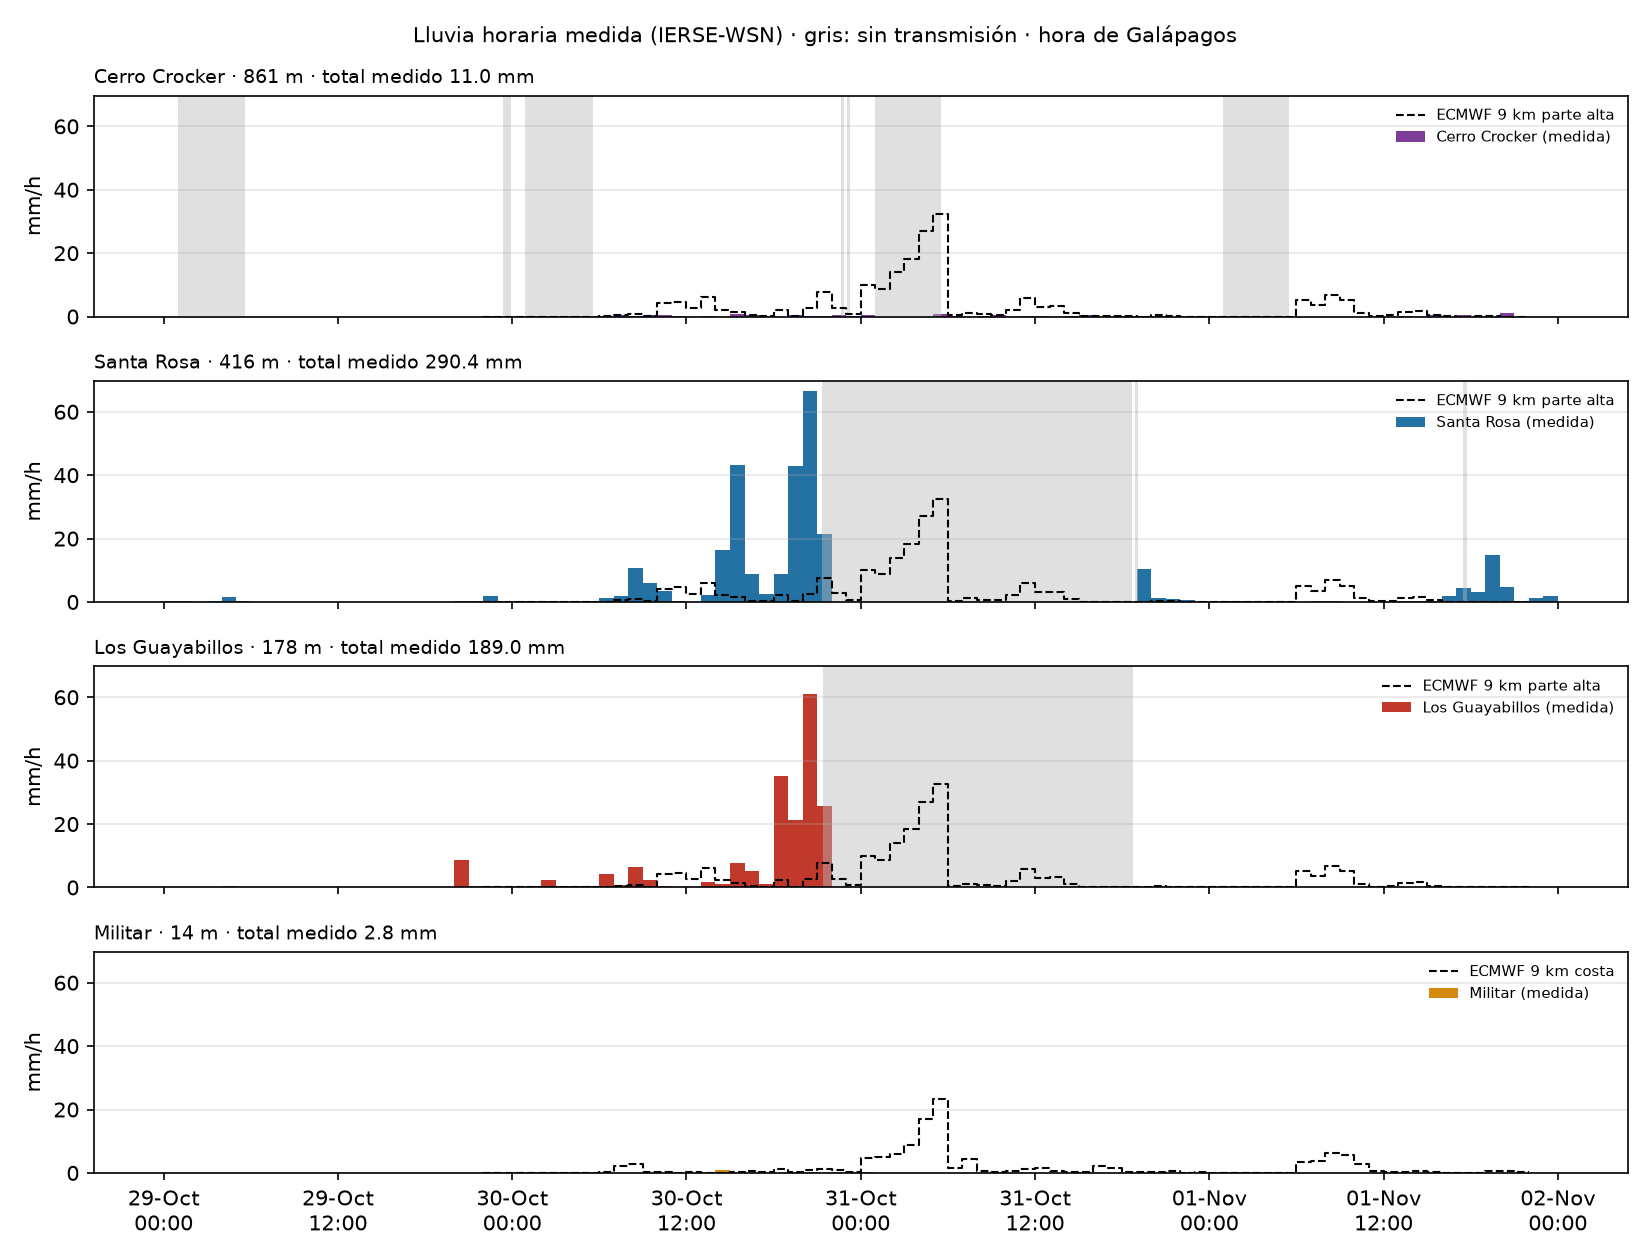
\includegraphics[width=0.72\linewidth]{f_hietograma.png}
  \caption{Lluvia horaria medida por la red IERSE-WSN del 29-oct al 1-nov-2026 (barras) y estimada por el ECMWF IFS de 9~km en la parte alta o en la costa (línea discontinua). En gris, los cortes de transmisión. Los totales del rótulo son los de toda la ventana, y son mínimos en Santa Rosa y Los Guayabillos. Hora de Galápagos. Generada por \texttt{clima/scripts/03\_evento.py}.}
  \label{fig:hietograma}
\end{figure}

\begin{figure}[t]
  \centering
  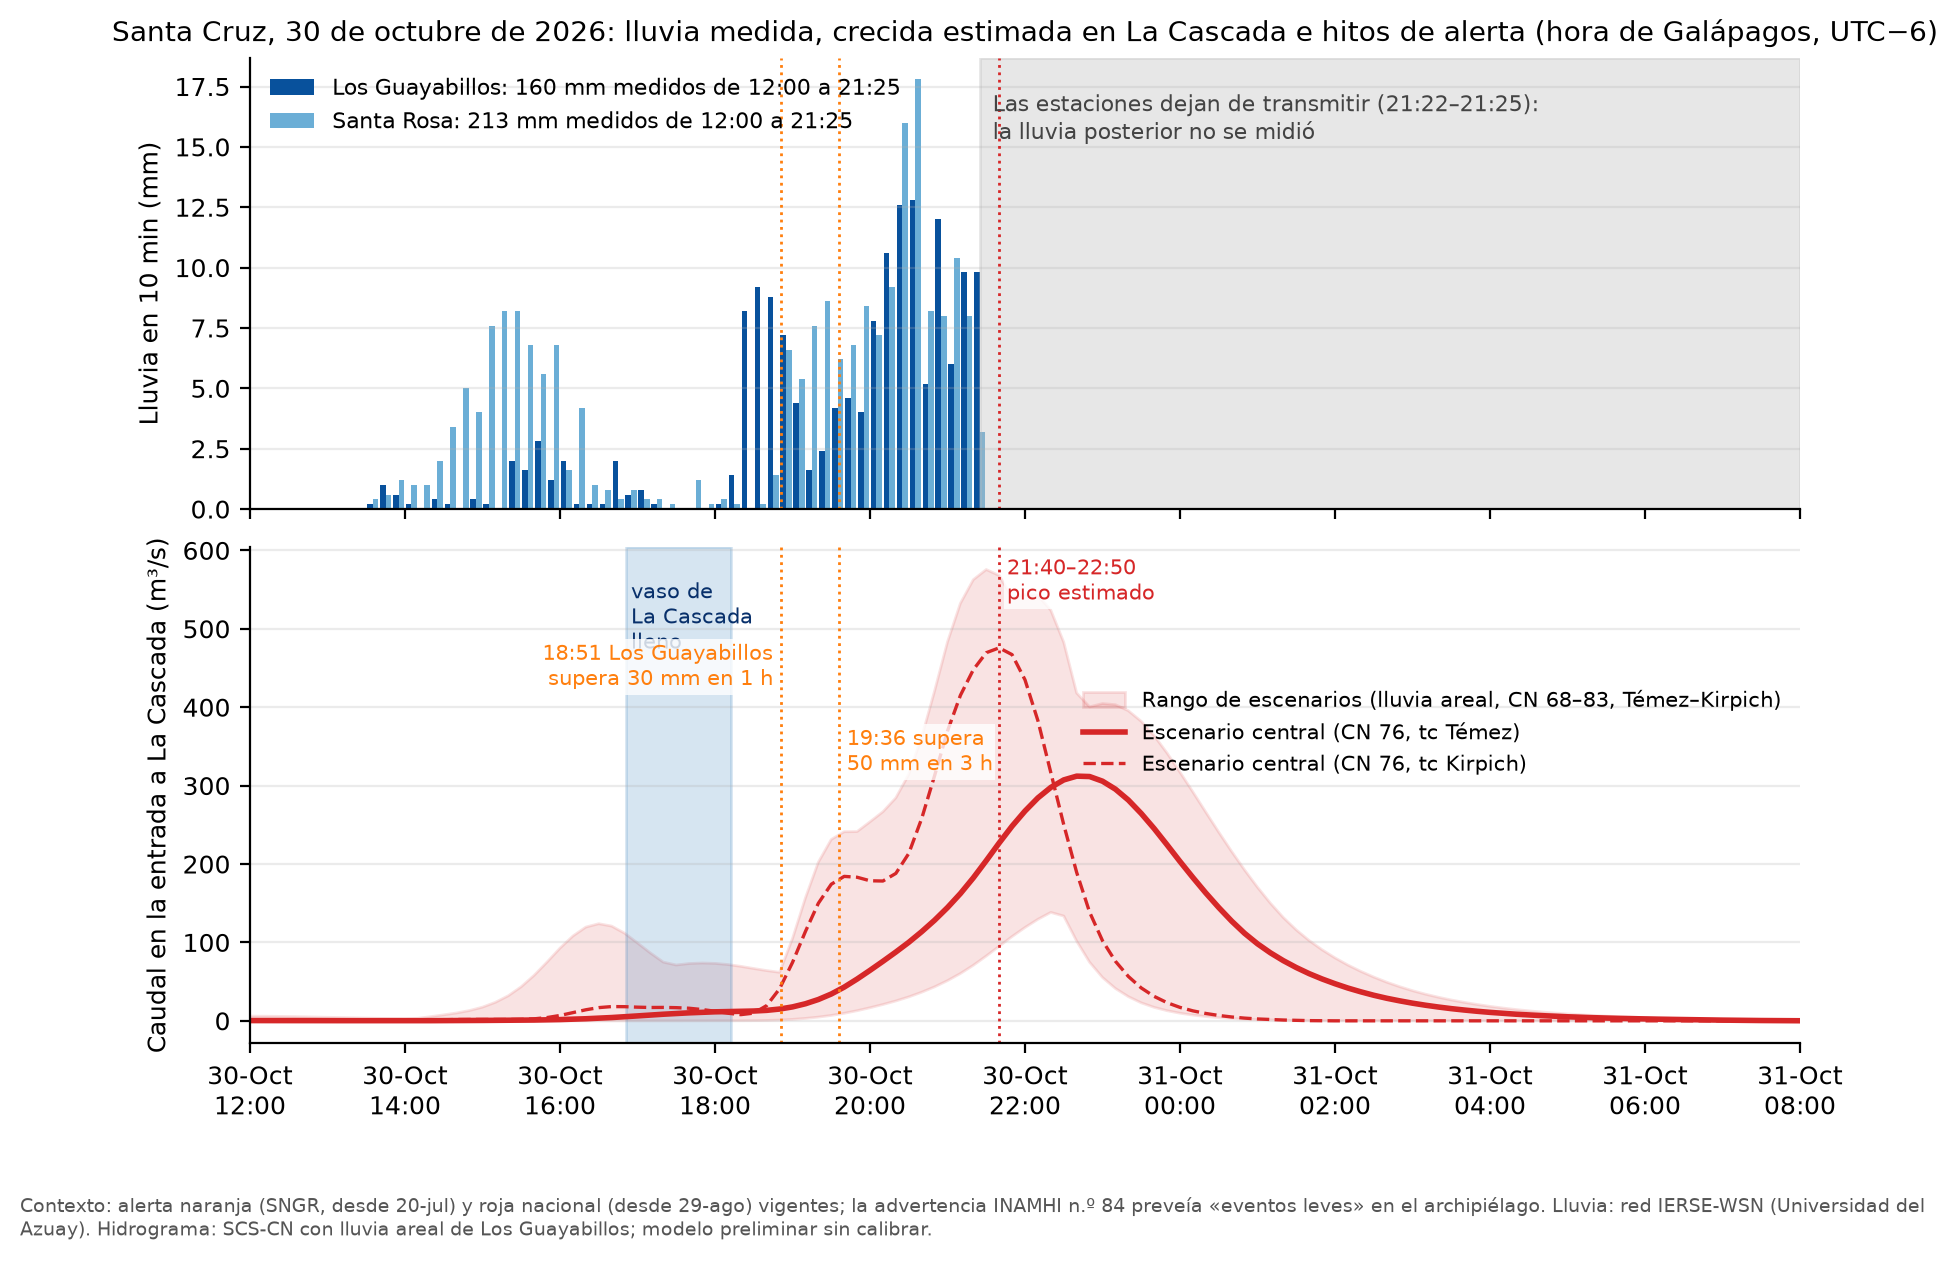
\includegraphics[width=0.8\linewidth]{cronologia_30oct.png}
  \caption{Arriba: lluvia medida cada 10~min en Los Guayabillos y Santa Rosa el 30-oct, con el corte de transmisión en gris. Abajo: caudal de entrada a La Cascada estimado con un modelo hidrológico preliminar (SCS-CN, sin calibrar) y los momentos en que se cruzaron los umbrales de la regla de alerta. El hidrograma es un \emph{modelo}; la lluvia, una \emph{medida}.}
  \label{fig:cronologia}
\end{figure}

\subsection{La costa de Santa Cruz: Puerto Ayora}
El M0191 del INAMHI, en la estación Charles Darwin (6~m, a 1,4~km de La Cascada), midió 118,5~mm el 30-oct y 110,5~mm el 31-oct, en días de Galápagos. En días continentales (UTC$-5$) las mismas horas suman 93,6 y 135,4~mm. La diferencia ilustra por qué la hora de cada fuente importa. Hora a hora (figura~\ref{fig:mareas}):
\begin{itemize}
  \item de 16:00 a 18:00 del 30-oct cayeron 44,6~mm, a la vez que el primer pulso de Santa Rosa;
  \item de 18:00 a 22:00, solo 7,4~mm: en la costa llovió poco cuando caía el máximo en la parte media;
  \item de 22:00 a 03:00 cayeron \textbf{135,1~mm} (24,7, 24,9, 36,8, 34,9 y 13,8~mm por hora). Es la lluvia que la red IERSE-WSN ya no registró.
\end{itemize}
La estación particular de Punta Estrada da la misma secuencia, con su máximo entre las 00:10 y las 01:10. Su sensor háptico mide un tercio de lo del M0191 (34,9 y 38,0~mm el 30 y el 31-oct), así que sirve para la hora pero no para la cantidad. No se sabe si la lluvia de 22:00 a 03:00 cayó también en la parte media de la cuenca de La Cascada. Si fue así, el barrio siguió recibiendo agua después del máximo que da el modelo 2D (informe 2026-06).

\subsection{San Cristóbal}
Las cuatro estaciones del GSC-USFQ en la parte alta de San Cristóbal sí cubren el evento, hora a hora, con el 99,7--99,8\,\% de las horas. Como el GSC no publica una licencia (\issue{46}), aquí solo se describen:
\begin{itemize}
  \item el 30-oct llovió de forma moderada toda la tarde y la noche, con 36--92~mm según la estación;
  \item el 31-oct midieron de 82 a 155~mm, más en las estaciones más altas;
  \item la hora más intensa fue de 08:00 a 10:00 del 31-oct, con un máximo de 39,1~mm en una hora. Es la misma mañana en que la SNGR sitúa el desborde de las cañadas, y en que el METAR del aeropuerto observó lluvia continua, moderada a ratos, de 08:00 a 14:00.
\end{itemize}
Ninguna de las cuatro estaciones está dentro de las cuencas que drenan a la ciudad o a El Progreso, y el pluviómetro M0221 del INAMHI en Puerto Baquerizo Moreno solo tiene datos desde el 2-nov. \textbf{La lluvia de la ciudad no se midió} (\issue{61}). Los datos horarios no permiten calcular intensidades en ventanas móviles ni en 5~min.

\subsection{Lo que estimaron los modelos}
En Santa Cruz los modelos fallaron en la hora, en la cantidad y en la intensidad (tabla~\ref{tab:modelos}; figuras~\ref{fig:hietograma} y~\ref{fig:medida}):
\begin{itemize}
  \item \textbf{Hora.} El ECMWF de 9~km situó su máximo entre las 05:00 y las 06:00 del 31-oct, unas 9~h después del máximo medido. En la ventana en que realmente llovió (14:00--22:00 del 30-oct) estimó entre el 7 y el 11\,\% de lo medido. Ningún modelo reprodujo los dos pulsos de la tarde y la noche.
  \item \textbf{Cantidad.} En 48~h, el ECMWF de 9~km (170--186~mm) quedó por debajo del mínimo medido en Santa Rosa ($\geq 251$~mm) y cerca del de Los Guayabillos ($\geq 179$~mm). La idea de que \enquote{el ECMWF sobrestima la lámina} no se sostiene.
  \item \textbf{Intensidad.} El ECMWF de 9~km dio la mitad de la intensidad horaria medida; los otros seis modelos, entre 13 y 74 veces menos.
  \item \textbf{Antes del evento.} Del 15 al 29-oct el ECMWF de 9~km dio unos 63~mm en las dos celdas, frente a 196~mm medidos en Santa Rosa y 18~mm en Los Guayabillos. El modelo no resuelve el contraste oeste--centro de la parte alta.
\end{itemize}
En San Cristóbal, los modelos daban entre 18 y 58~mm en Puerto Baquerizo Moreno para el 30 y el 31-oct. El ECMWF de 9~km pone la ciudad, el campus del GSC y El Progreso en una misma celda, y en la de El Junco dio 22,9~mm el 31-oct, unas siete veces menos que lo medido en esa estación. Entre las 07:00 y las 14:00 del 31 solo dio unos 6~mm.

\begin{table}[ht]
  \centering\small
  \caption{Lluvia medida frente a estimada en la celda de cada estación (mm). Modelos de Open-Meteo \citep{zippenfenig2023}, pedidos en hora de Galápagos. \enquote{Otros 6}: ECMWF 0,25°, GFS, ICON, JMA, Météo-France y UKMO.}
  \label{tab:modelos}
  \begin{tabularx}{\linewidth}{>{\raggedright\arraybackslash}Xccccc}
    \toprule
    Fuente & \makecell{30-oct\\14--22~h} & \makecell{Día\\30-oct} & \makecell{Día\\31-oct} & \makecell{30 + 31\\oct} & \makecell{Máx. 1~h\\(hora de inicio)} \\
    \midrule
    \textbf{Medido, Los Guayabillos} & \textbf{158,0} & $\boldsymbol{\geq 178{,}8}$ & $\geq 0$ (22\,\%) & $\boldsymbol{\geq 178{,}8}$ & \textbf{61,0 (30-oct, 20~h)} \\
    ECMWF 9~km, su celda & 17,1 & 39,8 & 129,8 & 169,6 & 32,5 (31-oct, 05~h) \\
    \addlinespace
    \textbf{Medido, Santa Rosa} & \textbf{210,6} & $\boldsymbol{\geq 237{,}6}$ & $\geq 13{,}4$ (21\,\%) & $\boldsymbol{\geq 251{,}0}$ & \textbf{66,4 (30-oct, 20~h)} \\
    ECMWF 9~km, su celda & 15,0 & 33,1 & 153,1 & 186,2 & 38,0 (31-oct, 05~h) \\
    \addlinespace
    Otros 6 modelos, mismas celdas & 1,1--7,2 & 2,8--15,6 & 0,2--30,5 & 3,0--41,8 & 0,9--4,6 \\
    \bottomrule
  \end{tabularx}
\end{table}

\begin{figure}[t]
  \centering
  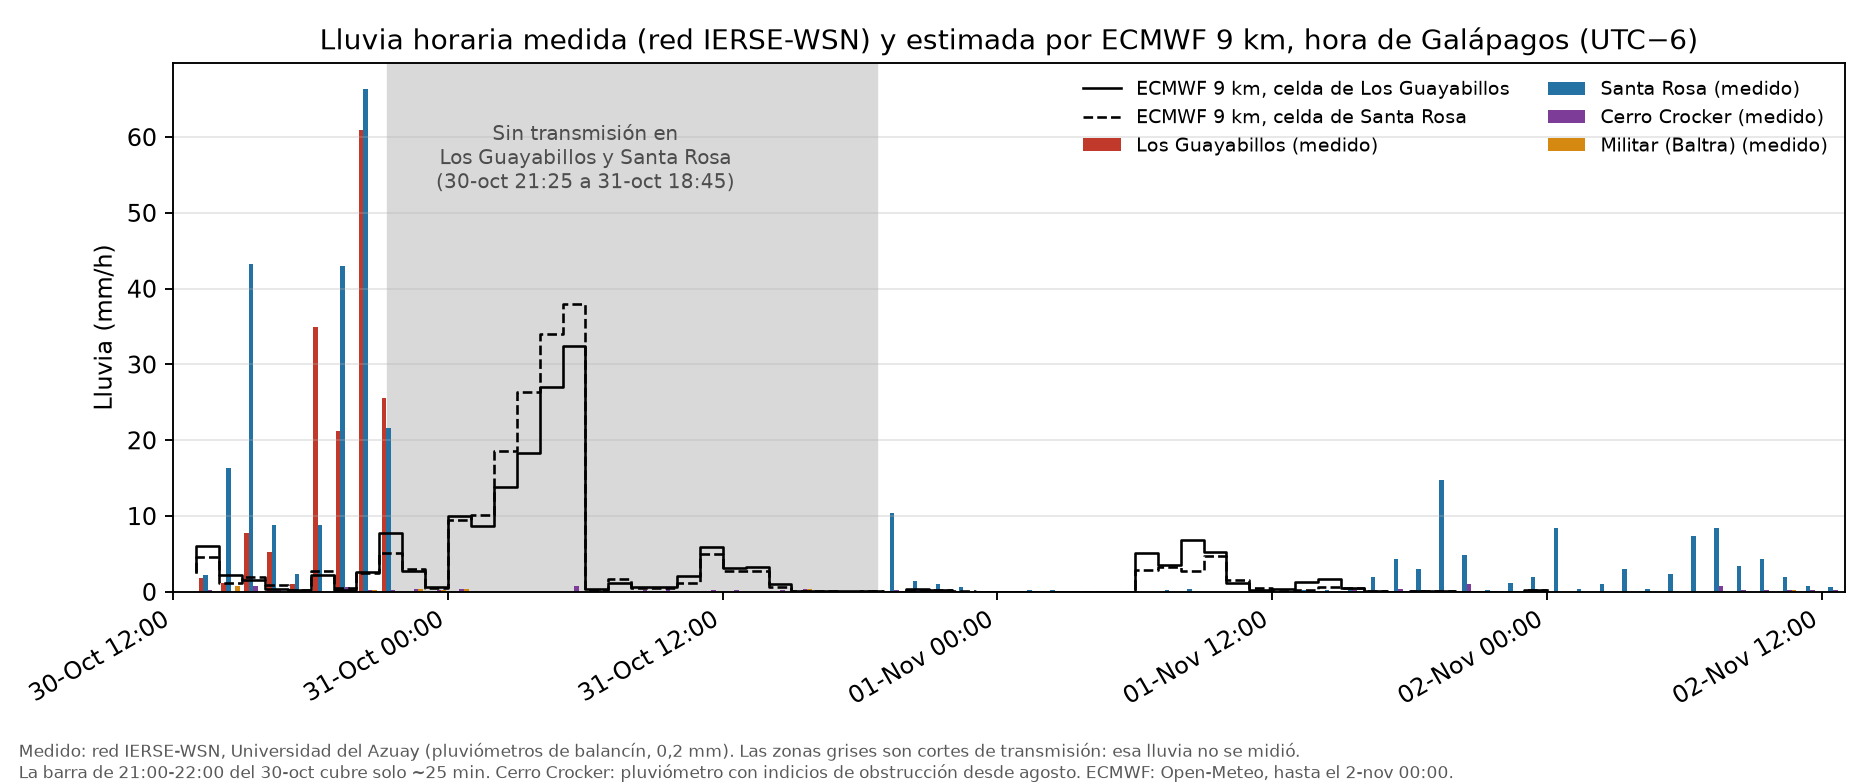
\includegraphics[width=0.84\linewidth]{f_lluvia_medida.png}
  \caption{Lluvia horaria medida por la red IERSE-WSN y estimada por el ECMWF IFS de 9~km, del 30-oct a las 12:00 al 2-nov a las 13:00. En gris, el corte de transmisión de Los Guayabillos y Santa Rosa. Generada por \texttt{geodatos/scripts/16\_lluvias\_ierse\_evento.py}.}
  \label{fig:medida}
\end{figure}


\subsection{El evento en la serie de la red}
El 30-oct es, de lejos, el mayor día de la serie de la red IERSE-WSN, del 23-abr al 2-nov-2026 (figura~\ref{fig:serie}). En total diario multiplica por 2,4--2,6 el segundo mayor día, y en intensidad horaria por 2,4--4,8 el segundo mayor valor. Octubre fue un mes húmedo: al menos 340~mm en Los Guayabillos y 521~mm en Santa Rosa, con 97,2~mm el 23-oct en Santa Rosa. Los cinco días previos al evento (25 al 29-oct) fueron casi secos, con 10--12~mm, así que el suelo no estaba saturado al empezar el 30. Sí debió de estarlo antes del segundo pulso: a las 18:00 ya habían caído unos 36~mm en Los Guayabillos y 98~mm en Santa Rosa desde la madrugada.

\begin{figure}[t]
  \centering
  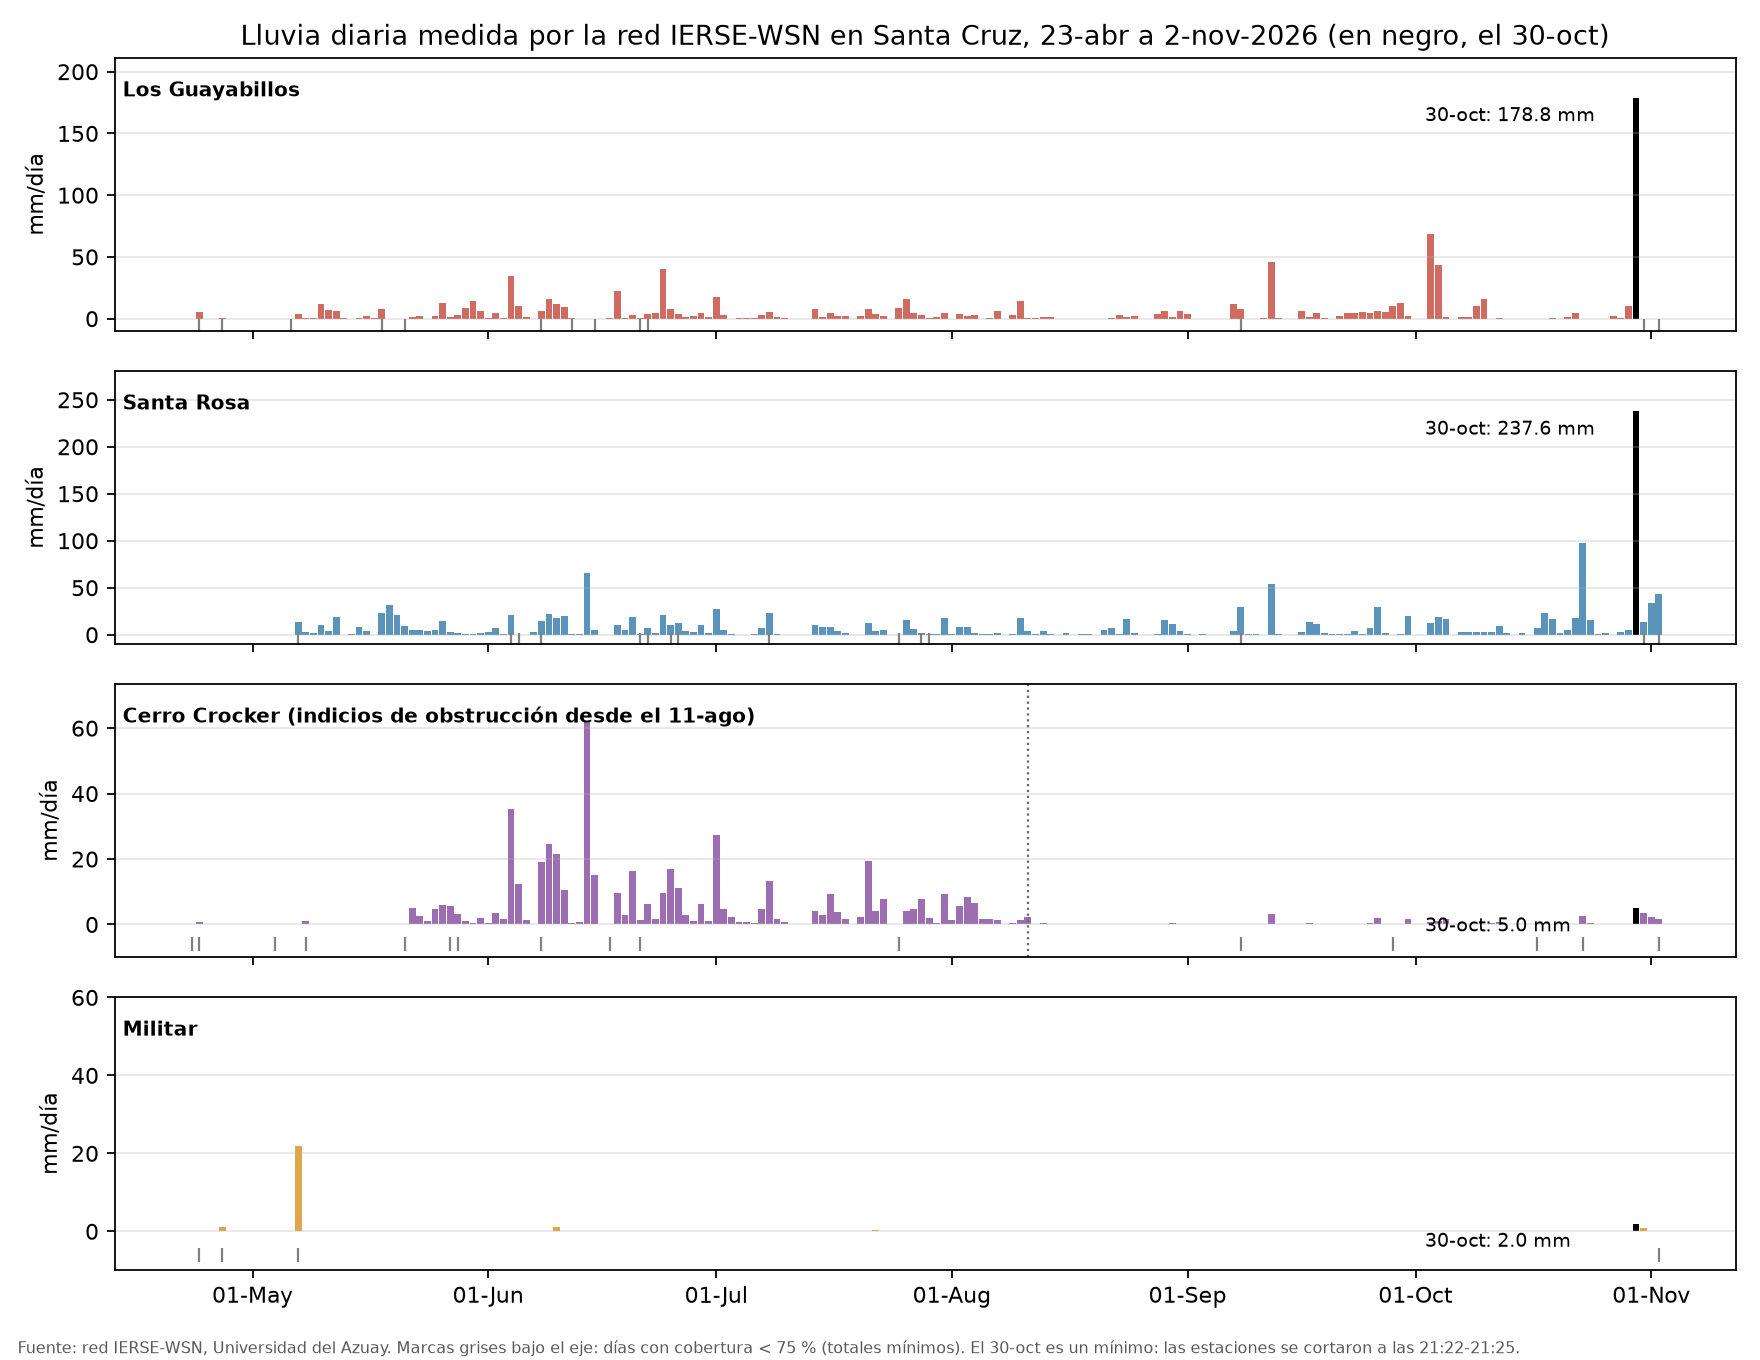
\includegraphics[width=0.66\linewidth]{f_lluvia_diaria_serie.png}
  \caption{Lluvia diaria medida por la red IERSE-WSN del 23-abr al 2-nov-2026, con el 30-oct en negro. Cerro Crocker deja de registrar lluvias apreciables desde el 11-ago (línea de puntos). La serie dura seis meses y no incluye ninguna estación cálida completa.}
  \label{fig:serie}
\end{figure}

\subsection{Calidad de los pluviómetros}\label{sec:calidad}
Dos estaciones de la red tienen dudas que solo una visita de campo puede resolver (\issue{56}):
\begin{itemize}
  \item \textbf{Cerro Crocker} cambió de comportamiento el 11 de agosto (tabla~\ref{tab:crocker}). Antes, en 33 días con 5~mm o más en Santa Rosa, registró al menos 1~mm en 32, y sumó el 85\,\% de lo de Santa Rosa. Después, solo 6 de 20 días comparables tuvieron 1~mm o más, sumó el 4\,\%, y no volvió a superar 1,2~mm en una hora. El patrón (tope de ${\approx}\,1$~mm/h y goteo regular) es el típico de un embudo parcialmente obstruido. Sus 5~mm del 30-oct no permiten concluir que la cumbre quedara seca.
  \item \textbf{Los Guayabillos} marcó 0,0~mm desde que volvió a transmitir (31-oct, 18:45) hasta el 2-nov, mientras Santa Rosa sumaba unos 90~mm. Puede estar obstruido, pero no es concluyente: ya hubo días con lluvia en Santa Rosa y nada en Los Guayabillos (23-oct: 97,2 frente a 0,0~mm), y la correlación diaria entre ambas es baja ($r = 0{,}37$, abril--octubre sin el evento).
  \item \textbf{Militar (Baltra)} marcó 0,0~mm mientras el METAR del aeropuerto, a unos 4~km, reportaba lluvia fuerte entre las 11:35 y las 13:00 del 30-oct. La lluvia pudo ser muy local, pero el dato es dudoso.
\end{itemize}

\begin{table}[ht]
  \centering\small
  \caption{Cerro Crocker frente a Santa Rosa y Los Guayabillos por periodos (mm). Red IERSE-WSN.}
  \label{tab:crocker}
  \begin{tabular}{lccccc}
    \toprule
    Periodo & \makecell{Crocker,\\total} & \makecell{Santa Rosa,\\total} & \makecell{Los Guayabillos,\\total} & \makecell{Crocker,\\máx. 1~h} & \makecell{Santa Rosa,\\máx. 1~h} \\
    \midrule
    23-abr a 31-may & 34,2 & 189,2 & 97,8 & 2,6 & 16,4 \\
    Junio & 296,6 & 290,6 & 190,4 & 23,2 & 13,2 \\
    Julio & 141,4 & 162,0 & 103,4 & 3,8 & 9,4 \\
    1 a 10-ago & 29,2 & 40,8 & 31,8 & 3,0 & 2,4 \\
    11 a 31-ago & \textbf{4,0} & 77,4 & 27,6 & 1,2 & 4,8 \\
    1-sep a 29-oct & \textbf{17,8} & 458,0 & 301,6 & \textbf{0,8} & 28,2 \\
    \bottomrule
  \end{tabular}
\end{table}

\subsection{¿Fue un récord?}
\textbf{Para octubre y noviembre, sí, con mucho margen} (tabla~\ref{tab:record}). El máximo diario de octubre o noviembre en Bellavista, a 223~m y a ${\approx}\,1{,}7$~km de Los Guayabillos, era de 59,5~mm (16-nov-1997): el 30-oct lo triplica. El mes de octubre multiplica por 5,3 la media de octubre de Bellavista. En Puerto Ayora, los 118,5~mm del M0191 superan los 104,3~mm del 2-oct-2023, pero son pluviómetros distintos y con días de lectura distintos.

\textbf{Para cualquier época del año, no necesariamente.} 178,8~mm ocuparían el 4.º lugar de la serie de Bellavista (el 1.º sin el episodio dudoso de 2008), y 237,6~mm, el 3.º. En 61 años de Puerto Ayora solo hay tres días por encima de 179~mm, todos en la estación cálida: 312~mm (31-mar-2022), 215~mm (22-feb-2024) y 186~mm (30-abr-1997). Los días más lluviosos de los grandes El Niño en Puerto Ayora fueron de 138~mm (1982--83) y 167~mm (1997--98); en Bellavista, de 130~mm (1997--98). Los $\geq 179$~mm de Los Guayabillos superan todos esos días. La intensidad horaria no se puede comparar: no hay series horarias históricas públicas en Santa Cruz.

\begin{table}[ht]
  \centering\small
  \caption{Lluvia del evento frente a los registros históricos de la FCD (mm).}
  \label{tab:record}
  \begin{tabularx}{\linewidth}{>{\raggedright\arraybackslash}p{4.3cm}>{\raggedright\arraybackslash}p{2.7cm}>{\raggedright\arraybackslash}p{2.7cm}>{\raggedright\arraybackslash}X}
    \toprule
    Indicador & Bellavista (FCD) & Puerto Ayora (FCD) & Evento 2026 \\
    \midrule
    Media de octubre (1991--2019/2020) & 63,7 & 10,9 & octubre: $\geq 340$ (LG), $\geq 521$ (SR) \\
    Octubre más lluvioso (1991--2019/2020) & 143,2 & 29,6 & --- \\
    Máx. diario de octubre o noviembre & 59,5 (1997) & 104,3 (2023) & $\geq 178{,}8$ (LG); $\geq 237{,}6$ (SR); 118,5 (M0191) \\
    Máx. diario de cualquier mes & 490,0 (2008)$^\dagger$; 164,1 (2005) & 312,0 (2022); 215,0 (2024) & --- \\
    \bottomrule
  \end{tabularx}
  \par\vspace{3pt}\raggedright\footnotesize LG: Los Guayabillos; SR: Santa Rosa (red IERSE-WSN, mínimos). $^\dagger$ Dato en duda (\issue{73}).
\end{table}

Que un evento así ocurra a finales de octubre, en plena estación de garúa, es coherente con El Niño en curso. El mar alrededor de Santa Cruz estuvo durante octubre entre 26,7 y 28,2~°C, con una anomalía de $+4{,}7$ a $+5{,}9$~°C \citep[OISST v2.1;][]{huang2021}. La región Niño 1+2 marcó $+5{,}4$~°C la semana del 28-oct (NOAA CPC), y el ERFEN declaró El Niño el 28 de agosto. En cambio, El Niño de 2015--16 dejó solo 225~mm en Puerto Ayora y 976~mm en Bellavista, con un máximo diario de 18 y 90~mm (\texttt{fcd\_nino.csv}): no todos los episodios traen lluvias extremas.


\subsection{Periodo de retorno}
La tabla~\ref{tab:gumbel} y la figura~\ref{fig:gumbel} dan el ajuste de Gumbel por momentos, el mismo que usa el tablero de clima. Con la serie de Puerto Ayora, 179~mm en un día vuelven cada ${\approx}\,21$ años y 238~mm cada ${\approx}\,78$. Con la de Bellavista el resultado depende de un solo dato:
\begin{itemize}
  \item con los 490~mm de marzo de 2008, $\beta = 64$~mm, y 179 y 238~mm vuelven cada 8 y 20 años;
  \item sin ese año, $\beta = 27$~mm, y vuelven cada 94 y más de 800 años.
\end{itemize}
El método de los momentos usa la desviación típica, muy sensible a un valor extremo; la máxima verosimilitud lo es menos. Con ella, en la serie completa de Bellavista, \texttt{29\_marburg\_darwin.py} da unos 23 años para 179~mm, y la GEV unos 16 (tabla~\ref{tab:retorno}).

\begin{table}[ht]
  \centering\small
  \caption{Gumbel por momentos de los máximos diarios anuales de la FCD (años con al menos el 80\,\% de días), calculado en este informe con el criterio de \texttt{estacionalidad.py}. Lámina para cada periodo de retorno y periodo de la lluvia medida el 30-oct-2026.}
  \label{tab:gumbel}
  \begin{tabular}{lccccccccc}
    \toprule
    Serie & Años & $\mu$ & $\beta$ & $x_{10}$ & $x_{25}$ & $x_{50}$ & $x_{100}$ & $T(179)$ & $T(238)$ \\
    \midrule
    Puerto Ayora & 61 & 45,6 & 44,1 & 145 & 187 & 218 & 248 & 21 & 78 \\
    Bellavista & 31 & 48,3 & 64,3 & 193 & 254 & 299 & 344 & 8 & 20 \\
    Bellavista sin 2008 & 30 & 56,4 & 27,0 & 117 & 143 & 162 & 180 & 94 & ${>}\,800$ \\
    \bottomrule
  \end{tabular}
  \par\vspace{3pt}\raggedright\footnotesize Láminas en mm y periodos en años. $T(118{,}5)$, la lluvia del M0191 en Puerto Ayora: 5,7 años con la serie de Puerto Ayora.
\end{table}

\begin{figure}[t]
  \centering
  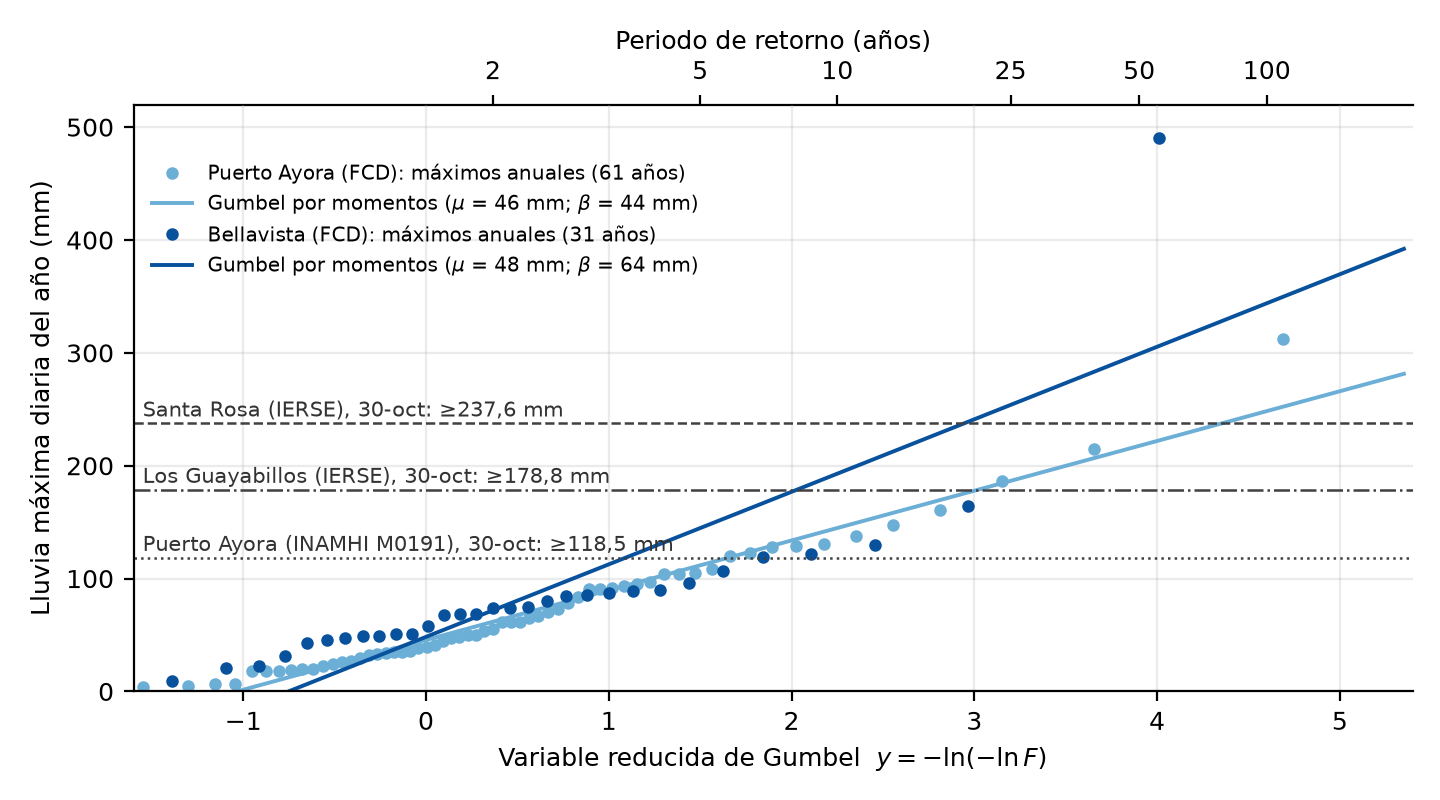
\includegraphics[width=0.74\linewidth]{gumbel_fcd.png}
  \caption{Máximos diarios anuales de la FCD en papel de Gumbel (posiciones de Gringorten) y su ajuste por momentos, con la lluvia medida el 30-oct-2026 (mínimos). El punto aislado de Bellavista es el dato dudoso de marzo de 2008 (490~mm), que inclina toda la recta. Figura de \texttt{informes/2026-03-lluvia-clima/figuras.py}; datos de la FCD (CC BY-NC-SA).}
  \label{fig:gumbel}
\end{figure}

El reanálisis GAR da periodos más cortos, de 7 a 9 años para 179~mm en las celdas de Bellavista y Los Guayabillos (tabla~\ref{tab:retorno}; figura~\ref{fig:maxanual}). En la celda de Puerto Ayora reproduce bien el nivel medio de los máximos (68,8~mm frente a 76,5~mm medidos; cociente 0,90) y el total anual (465 frente a 495~mm). Acierta qué años son lluviosos (Spearman de 0,81 en los totales anuales), pero no los días concretos: la correlación de los máximos anuales es de 0,51. En la celda de Bellavista sobrestima los máximos (cociente 1,08) y subestima el total (0,71). En la de Santa Rosa supera los 179~mm en 21 de 46 años: en el modelo es la zona de lluvias extremas más intensas de la isla, pero no hay ninguna serie medida larga allí para comprobarlo.

\begin{table}[ht]
  \centering\small
  \caption{Periodo de retorno indicativo (años, régimen anual) de la lluvia diaria del 30-oct según la fuente y el método.}
  \label{tab:retorno}
  \begin{tabular}{llccc}
    \toprule
    Fuente & Método & Años & 179~mm & 238~mm \\
    \midrule
    Pluviómetro de Bellavista (FCD) & Gumbel MV (GEV) & 31 & ${\approx}\,23$ (${\approx}\,16$) & ${\approx}\,110$ (${\approx}\,40$) \\
    & Gumbel momentos & 31 & 8 & 20 \\
    & Gumbel momentos, sin 2008 & 30 & 94 & ${>}\,800$ \\
    Pluviómetro de Puerto Ayora (FCD), costa & Gumbel MV (GEV) & 61 & ${\approx}\,33$ (${\approx}\,18$) & ${\approx}\,150$ (${\approx}\,40$) \\
    & Gumbel momentos & 61 & 21 & 78 \\
    GAR, celdas de Bellavista y Los Guayabillos & Gumbel MV & 46 & ${\approx}\,7$--9 & ${\approx}\,20$--40 \\
    \bottomrule
  \end{tabular}
  \par\vspace{3pt}\raggedright\footnotesize MV: máxima verosimilitud (\texttt{29\_marburg\_darwin.py} y estudio de Santa Cruz). Momentos: este informe. GAR es lluvia modelada.
\end{table}

\begin{figure}[t]
  \centering
  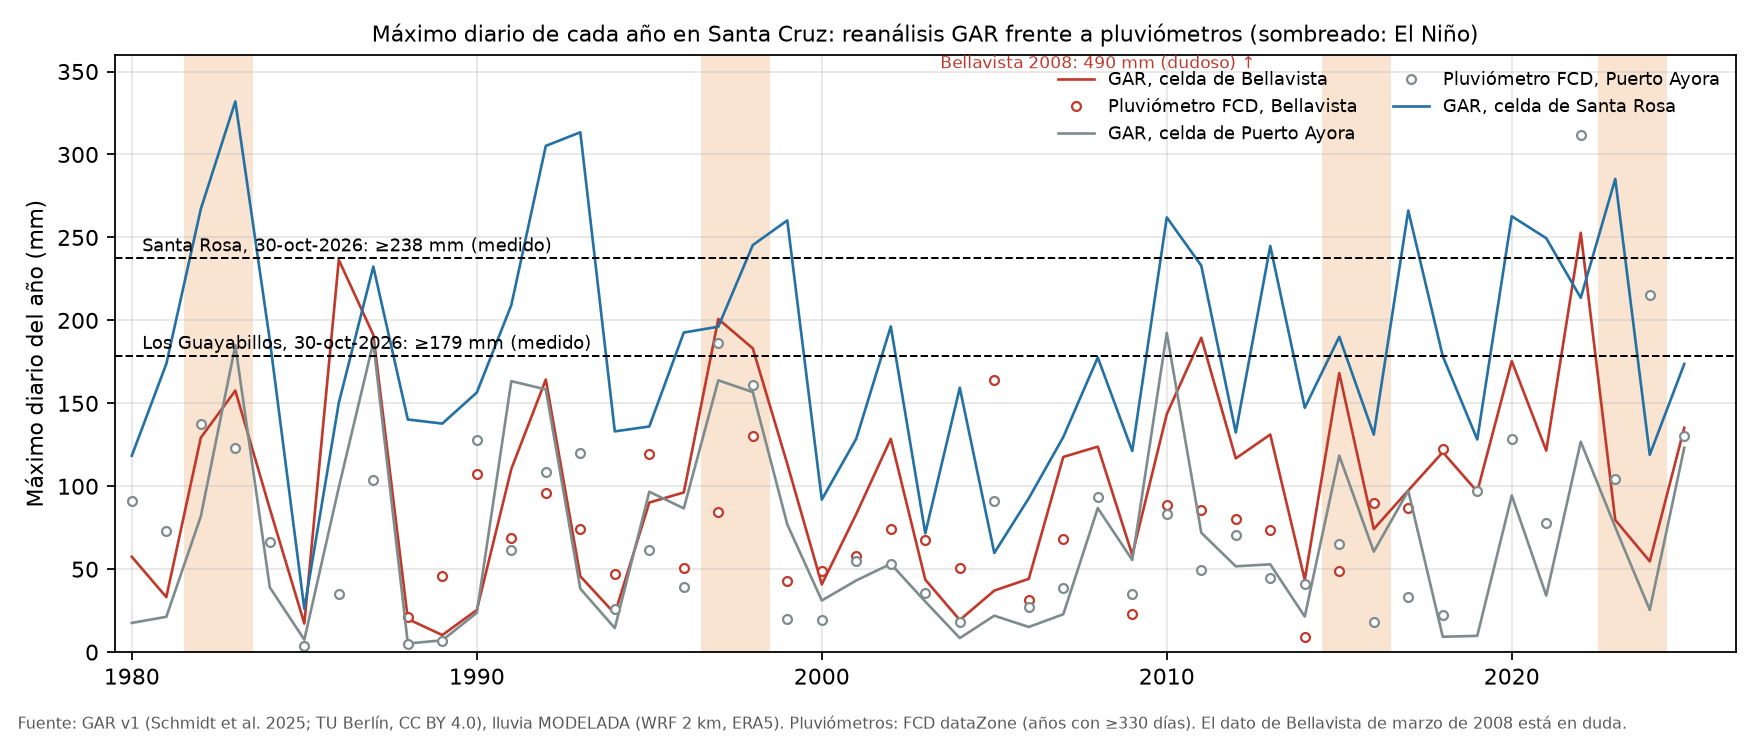
\includegraphics[width=0.82\linewidth]{marburg_max_anual_santa_cruz.png}
  \caption{Máximo diario de cada año en Santa Cruz: reanálisis GAR (lluvia \emph{modelada}, celdas de 2~km) frente a los pluviómetros de la FCD (lluvia \emph{medida}). Sombreado: años El Niño. Líneas discontinuas: lluvia medida el 30-oct-2026. Generada por \texttt{geodatos/scripts/29\_marburg\_darwin.py}.}
  \label{fig:maxanual}
\end{figure}

\textbf{La lluvia y la cota.} En GAR, el total anual crece con la cota mucho más que el máximo diario (figura~\ref{fig:gradiente}). En el conjunto de Santa Cruz, entre la franja de 0--100~m y la de 600--700~m, el total se multiplica por 2,7 y la media de los máximos diarios por 1,8. En San Cristóbal, a lo largo del transecto de barlovento, el máximo diario casi no cambia con la cota (factor de 0,97 a 1,04), aunque el total crezca 1,4 veces. GAR no está validado en San Cristóbal: en la costa da ${\approx}\,1270$~mm/año, frente a los ${\approx}\,500$ publicados \citep{paltan2021}, es decir, unas 2,5 veces demasiado (figura~\ref{fig:gar-scb}).

\begin{figure}[t]
  \centering
  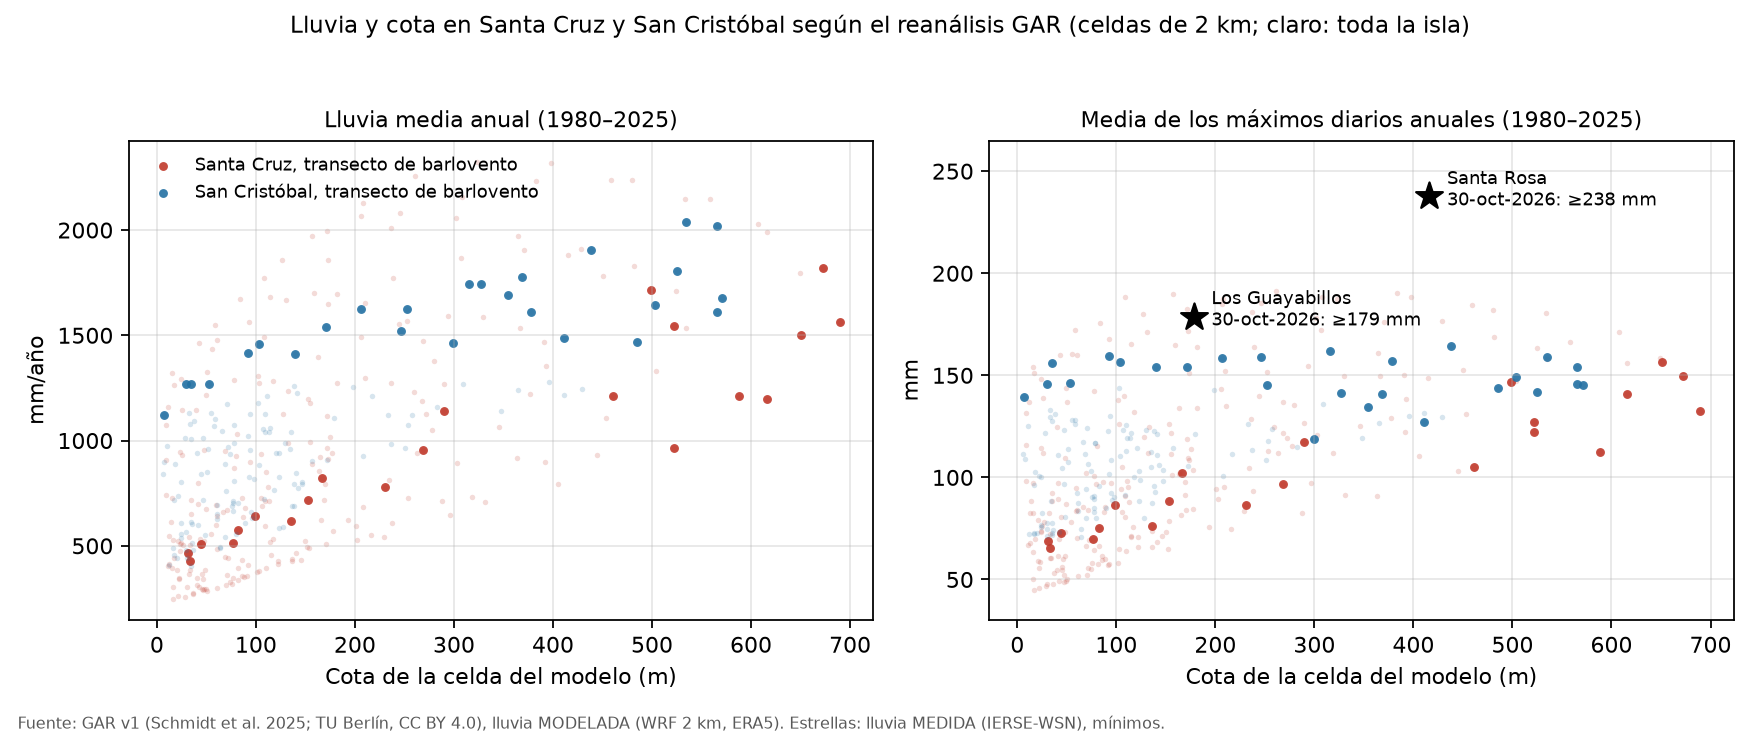
\includegraphics[width=0.8\linewidth]{marburg_gar_gradiente.png}
  \caption{Lluvia media anual y media de los máximos diarios anuales frente a la cota de la celda en el reanálisis GAR (1980--2025). Puntos fuertes: transectos de barlovento; claros: todas las celdas de cada isla. Las estrellas son la lluvia \emph{medida} el 30-oct-2026 (mínimos).}
  \label{fig:gradiente}
\end{figure}

\begin{figure}[t]
  \centering
  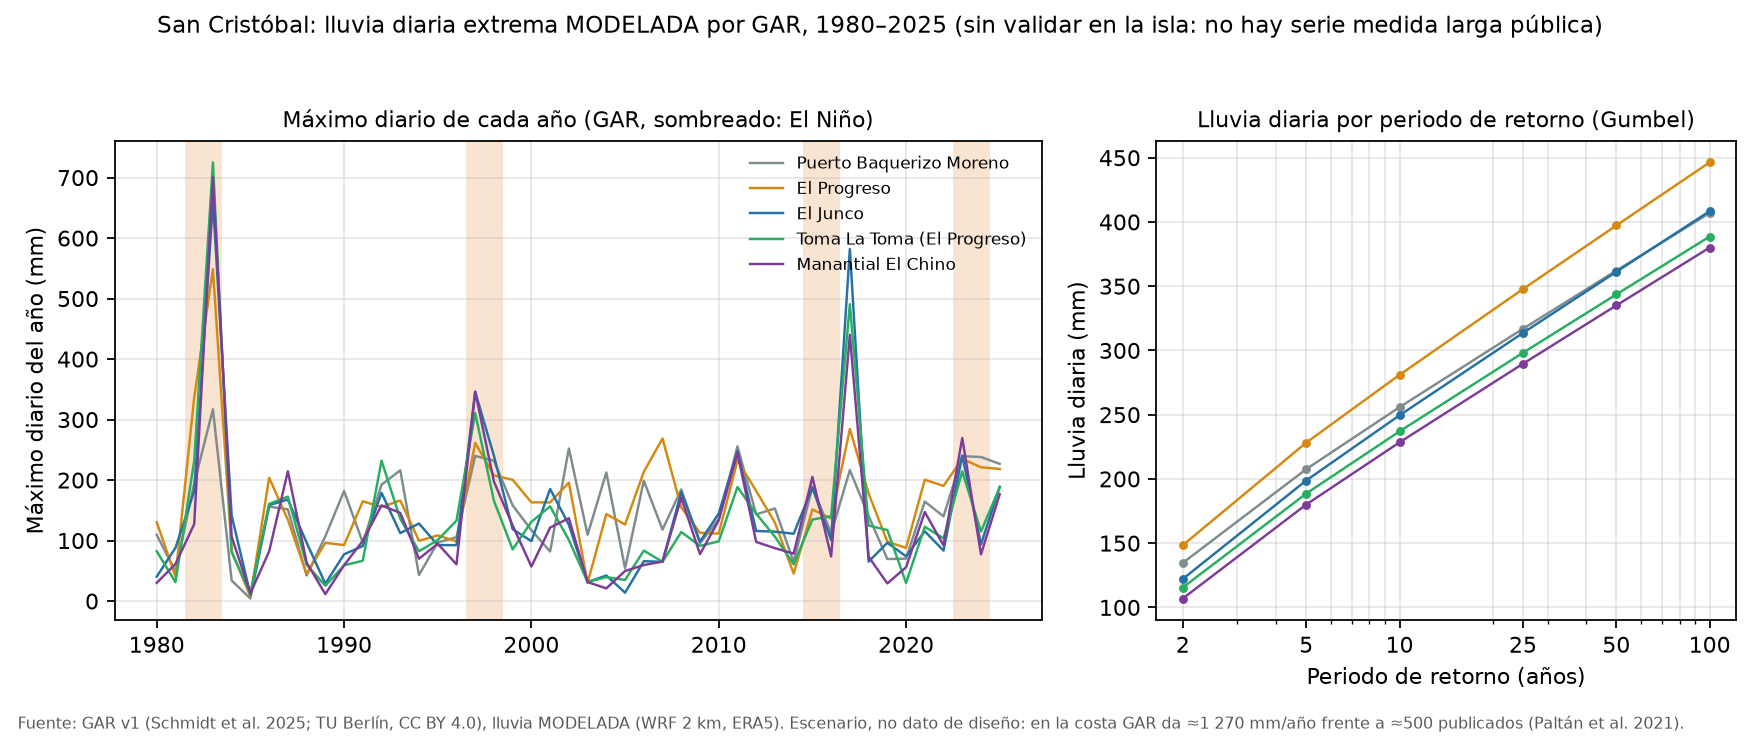
\includegraphics[width=0.8\linewidth]{marburg_gar_san_cristobal.png}
  \caption{San Cristóbal: lluvia diaria extrema modelada por GAR, 1980--2025, en Puerto Baquerizo Moreno, El Progreso, El Junco y las tomas de agua. Es un reanálisis sin validar en la isla, unas 2,5 veces más húmedo que los totales publicados en la costa: sus milímetros no deben leerse como medidas.}
  \label{fig:gar-scb}
\end{figure}

\textbf{Climatología mensual.} En la costa, octubre es de los meses más secos: la media de Puerto Ayora es de 10,9~mm (1991--2020). En Bellavista la media de octubre es de 63,7~mm, y la estación más lluviosa va de enero a mayo, con la garúa el resto del año.


\subsection{La lluvia y el nivel del mar}
\textbf{La marea astronómica.} El ajuste con UTide reproduce el nivel fuera de muestra con un error cuadrático medio de 1,8~cm en Puerto Ayora y 2,2~cm en Baltra, sobre mareas de 1,8--2,1~m (tabla~\ref{tab:mareas}). La marea es semidiurna: M2 aporta 0,65~m de amplitud en Puerto Ayora y 0,73~m en Baltra, con fases casi iguales (246° y 245°). El mareógrafo IOC queda 1,8~cm por encima del cero del UHSLC (dispersión de 0,9~cm en 679~h de solape).

\begin{table}[ht]
  \centering\small
  \caption{Constantes armónicas principales (amplitud en m) y validación fuera de muestra (julio--septiembre de 2026). UTide sobre las series horarias del UHSLC, 2022--2026.}
  \label{tab:mareas}
  \begin{tabular}{lcccccc}
    \toprule
    Mareógrafo & M2 & S2 & N2 & K1 & \makecell{Fase M2\\(°)} & \makecell{Error cuadrático\\medio (cm)} \\
    \midrule
    Puerto Ayora (Academy Bay) & 0,646 & 0,190 & 0,140 & 0,091 & 246,4 & 1,8 \\
    Baltra & 0,726 & 0,194 & 0,159 & 0,083 & 244,7 & 2,2 \\
    \bottomrule
  \end{tabular}
\end{table}

\textbf{El traslado a Puerto Baquerizo Moreno.} Según Open-Meteo Marine, la onda M2 de Puerto Baquerizo Moreno es un 9,8\,\% mayor que la de Puerto Ayora ($r = 1{,}098$) y llega 0,4~min después ($\tau \approx 0$). En Puerto Ayora el modelo da una amplitud de M2 muy parecida a la del mareógrafo (0,634 frente a 0,646~m), pero su fase difiere en 15° (231° frente a 246°), unos 31~min. Por eso solo se usan las diferencias entre las dos celdas del modelo, no sus valores absolutos. El resultado es coherente con lo observado en la serie del modelo: la pleamar ocurre a la misma hora (${\pm}\,15$~min) y con una altura parecida (${\pm}\,10$\,\%) en las dos bahías. Es una estimación sin validar: no hay ninguna medida del nivel del mar en Puerto Baquerizo Moreno.

\textbf{El Niño en el nivel del mar.} El nivel medio mensual en Puerto Ayora pasó de $-7$~cm en septiembre de 2025 a $+30$~cm en septiembre de 2026, respecto del nivel medio de 2017--2024 (figura~\ref{fig:anomalia}). Durante el evento, el residuo no astronómico fue de $+0{,}48$ a $+0{,}51$~m, y el 2-nov era de $+41$~cm.

\begin{figure}[t]
  \centering
  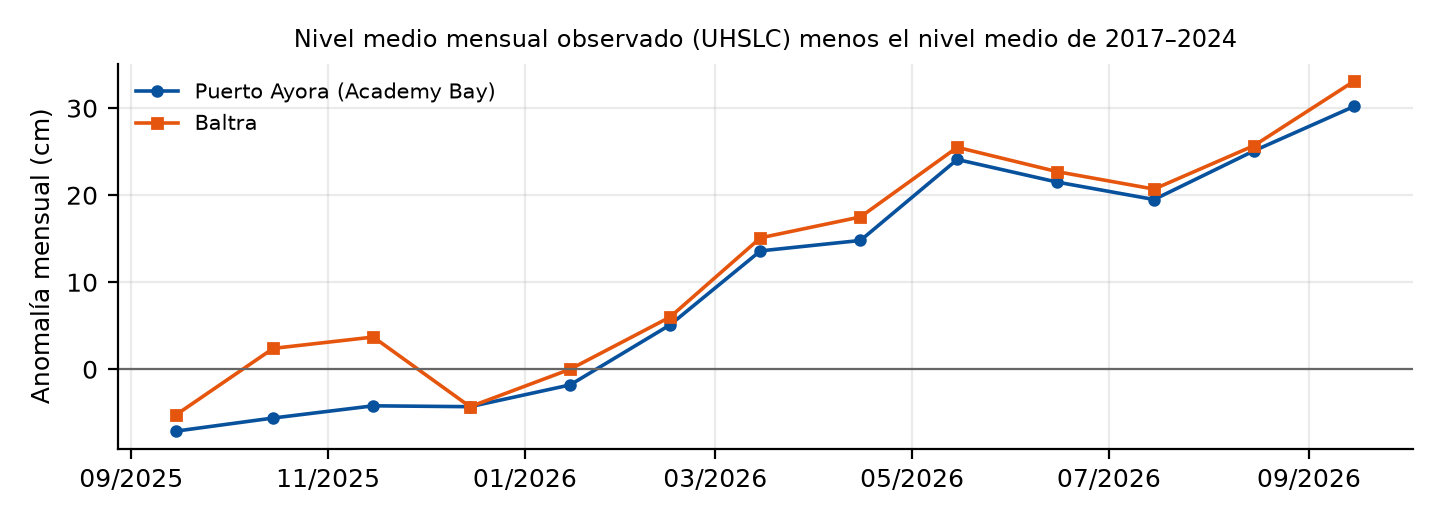
\includegraphics[width=0.7\linewidth]{anomalia_nivel_mar.png}
  \caption{Nivel medio mensual observado en Puerto Ayora y Baltra (UHSLC) menos el nivel medio de 2017--2024. La subida desde febrero de 2026 es la señal de El Niño en el nivel del mar. Figura de \texttt{informes/2026-03-lluvia-clima/figuras.py} con \texttt{geodatos/datos/mareas/resumen\_mareas.json}.}
  \label{fig:anomalia}
\end{figure}

\textbf{La marea durante el evento} (tabla~\ref{tab:marea-evento}; figura~\ref{fig:mareas}). La pleamar del 30-oct fue a las 17:50, con 1,21~m de marea astronómica. El máximo de lluvia en la parte media (20:30--20:40) y la llegada del agua al centro de La Cascada en el modelo 2D (20:50) ocurrieron con la marea \emph{bajando}, a unas 3~h de la pleamar. El pico de salida del agua al mar en el modelo (22:30) fue con el nivel observado a solo $+0{,}05$~m, a 1,5~h de la bajamar. El rango de marea en 25~h (1,67~m) fue intermedio, ni sicigia ni cuadratura plenas. El máximo de la lluvia costera del M0191 (00:30 del 31-oct) cayó cerca de la bajamar. \textbf{La marea no agravó el desagüe de La Cascada}, aunque el nivel estaba unos 0,5~m por encima de la marea astronómica.

El modelo 2D de Santa Cruz (informe 2026-06) usa un mar fijo a $+0{,}75$~m. El máximo observado entre las 20:00 y las 24:00 fue de $+0{,}82$~m, y a las 22:00, de $+0{,}17$~m. El nivel fijo es, por tanto, conservador para el pico de salida al mar, aunque no para las horas cercanas a la pleamar.

\begin{table}[ht]
  \centering\small
  \caption{Nivel del mar en Puerto Ayora en los momentos clave del 30-oct-2026 (m sobre el nivel medio de 2017--2024). Obs.: observado (mareógrafo IOC). Astr.: marea astronómica. Residuo: diferencia. 2D: modelo 2D del informe 2026-06.}
  \label{tab:marea-evento}
  \begin{tabularx}{\linewidth}{>{\raggedright\arraybackslash}Xccccl}
    \toprule
    Momento & Hora & Obs. & Astr. & Residuo & Fase de la marea \\
    \midrule
    Máx. 60~min, Los Guayabillos & 20:30 & 0,67 & 0,18 & 0,49 & bajando (pleamar $+2{,}7$~h) \\
    Máx. 60~min, Santa Rosa & 20:40 & 0,61 & 0,12 & 0,48 & bajando (pleamar $+2{,}8$~h) \\
    Llegada del agua a La Cascada (2D) & 20:50 & 0,56 & 0,06 & 0,49 & bajando (pleamar $+3{,}0$~h) \\
    Pico de salida al mar (2D) & 22:30 & 0,05 & $-0{,}46$ & 0,51 & bajando (bajamar $-1{,}5$~h) \\
    Máx. 1~h, M0191 & 00:30$^{*}$ & $-0{,}09$ & $-0{,}60$ & 0,51 & cerca de la bajamar \\
    \bottomrule
  \end{tabularx}
  \par\vspace{3pt}\raggedright\footnotesize $^{*}$ Del 31-oct. Fuente: \texttt{geodatos/estudios/santa-cruz/datos/lluvia\_mareas\_eventos.csv}.
\end{table}

\begin{figure}[t]
  \centering
  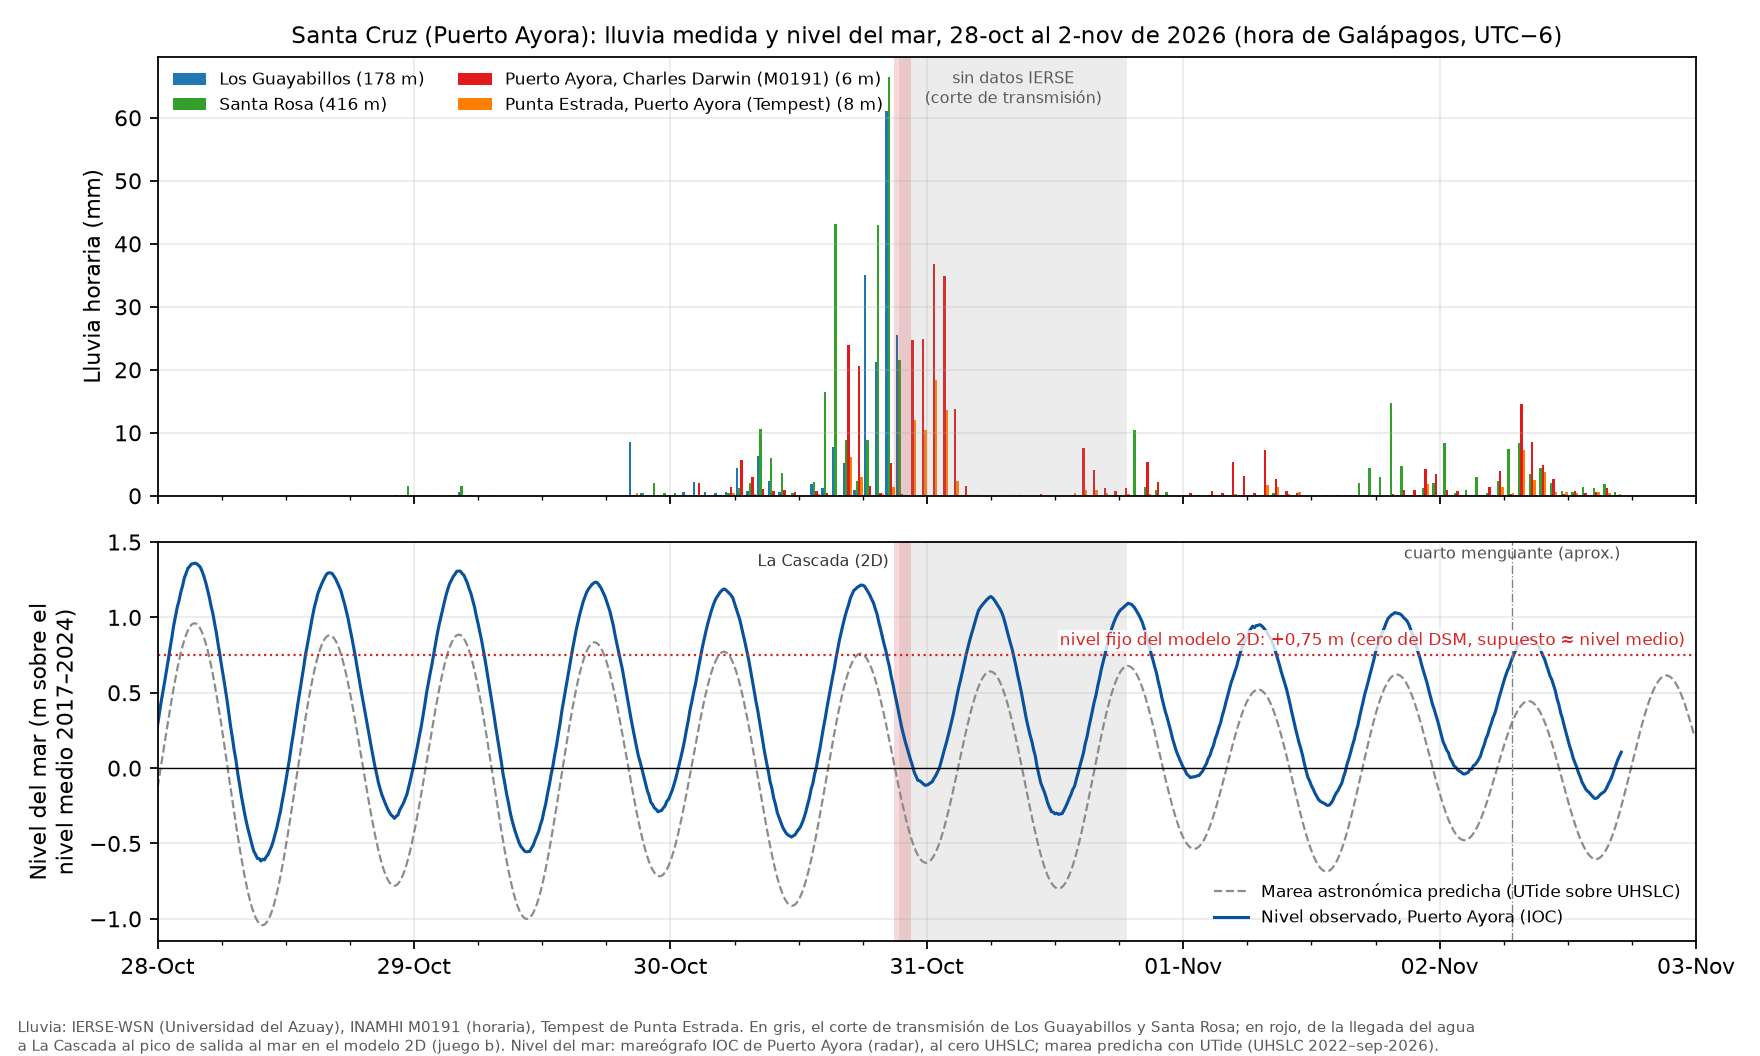
\includegraphics[width=0.8\linewidth]{mareas_lluvia_28oct_2nov.png}
  \caption{Santa Cruz, 28-oct a 2-nov-2026. Arriba: lluvia horaria medida por la red IERSE-WSN, el M0191 del INAMHI y la estación particular de Punta Estrada; en gris, el corte de IERSE; en rojo, desde la llegada del agua a La Cascada hasta el pico de salida al mar en el modelo 2D. Abajo: nivel observado en Puerto Ayora (IOC) y marea astronómica predicha (UTide sobre UHSLC), con el nivel fijo del modelo 2D. Generada por \texttt{geodatos/scripts/30\_lluvia\_mareas.py}.}
  \label{fig:mareas}
\end{figure}

% =====================================================================
\section{Discusión y limitaciones}

\textbf{Lo que no se midió pesa tanto como lo que se midió.} El corte de la red empezó cuando llovía a 38--55~mm/h, y la costa recibió 135~mm más después de las 22:00 sin que se sepa si esa lluvia llegó a la parte media. Cualquier modelo hidrológico del evento arrastra esa incertidumbre en la cola del hidrograma. Los registros en memoria de las estaciones, si existen, o las series de 10~min del proyecto DARWIN podrían cerrar ese hueco (\issue{62}, \issue{76}).

\textbf{Los modelos globales no sirven como medida del evento.} Ni el mejor, el ECMWF de 9~km, reprodujo la hora, la intensidad ni el contraste espacial: su lámina de 48~h se acercó a lo medido, pero con el máximo nueve horas tarde. Su posible uso como señal probabilística, y no como cantidad, se evalúa en el informe 2026-08.

\textbf{El periodo de retorno es un orden de magnitud.} Según la serie y el método, 179~mm en un día vuelven cada 7 a 94 años. La mayor incertidumbre no es estadística sino de datos: un solo valor dudoso de Bellavista multiplica por más de diez el periodo con el método de los momentos, y afecta igual a las láminas que publica el tablero de clima para esa estación. Además, la serie mezcla años El Niño y normales; los valores medidos son mínimos y cayeron en unas 7~h, no en 24; Santa Rosa está a otra cota que Bellavista; y los días de la FCD y de GAR no coinciden con el día natural. Para la intensidad horaria no hay curvas IDF publicadas en Santa Cruz; el informe 2026-02 propone unas provisionales.

\textbf{GAR es lluvia modelada.} Sirve para el nivel medio de los máximos y para comparar años, pero su cola alta es más pesada que la medida en Santa Cruz, y en la costa de San Cristóbal está unas 2,5 veces por encima de los totales publicados.

\textbf{La calidad de la red y del nivel del mar.} Dos de las cuatro estaciones de IERSE-WSN tienen dudas de funcionamiento y una tercera es dudosa (\issue{56}); sus balancines subestiman además las intensidades altas. El nivel del mar está medido en Puerto Ayora, pero en Puerto Baquerizo Moreno es una estimación sin validar. El cero del mareógrafo aún no está enlazado con el datum del DSM ni con el del IGM (\issue{75}), así que comparar el nivel del mar con cotas del terreno exige cautela.

% =====================================================================
\section{Conclusiones y trabajo futuro}
\begin{enumerate}
  \item El 30-oct se midieron al menos 178,8~mm en Los Guayabillos y 237,6~mm en Santa Rosa, con 61--66~mm en una hora de reloj, 64--73~mm en 60~min móviles y 138--139~mm en 3~h. Son mínimos: la red dejó de transmitir a las 21:22--21:25 durante 21,3~h, y en la costa cayeron 135~mm más entre las 22:00 y las 03:00.
  \item En San Cristóbal la lluvia más intensa fue la mañana del 31-oct en la parte alta, con un máximo de 39,1~mm en una hora. La lluvia de la ciudad no se midió.
  \item Los modelos globales situaron el máximo unas 9~h tarde y con, como mucho, la mitad de la intensidad horaria. No sirven como estimación cuantitativa de un evento convectivo en las islas.
  \item Para octubre y noviembre el evento no tiene precedente en más de 30 años de registros cercanos. En régimen anual es de años a decenas de años, con una incertidumbre dominada por la calidad de la serie de Bellavista.
  \item La marea estaba bajando cuando el agua llegó a La Cascada y no agravó el desagüe, aunque El Niño mantenía el mar unos 0,5~m por encima de la marea astronómica.
\end{enumerate}

Quedan pendientes:
\begin{itemize}
  \item recuperar la lluvia del corte de la red IERSE-WSN y conocer su causa (\issue{62});
  \item revisar en campo los pluviómetros de Cerro Crocker y Los Guayabillos (\issue{56});
  \item la serie original de Bellavista y el episodio de marzo de 2008 (\issue{73});
  \item las series del proyecto DARWIN del 15-oct al 2-nov y el permiso para publicar derivados (\issue{76});
  \item la lluvia de la ciudad y de 5--10~min en San Cristóbal (\issue{61}) y la licencia de los datos del GSC (\issue{46});
  \item la lectura diaria de la estación Charles Darwin del 15-oct al 2-nov (\issue{63});
  \item un mareógrafo o una serie de mareas en Puerto Baquerizo Moreno (\issue{13}) y el enlace del mareógrafo de Puerto Ayora con el datum del terreno (\issue{75});
  \item renombrar los scripts con prefijo duplicado (\issue{57}).
\end{itemize}

\section*{Disponibilidad de datos y código}
{\small Todo el procesamiento es reproducible desde el repositorio público \emph{mayait/sosgalapagos-datos}. Los endpoints de las fuentes no se publican: viven en \texttt{clima/privado/}, fuera del control de versiones.
\begin{itemize}
  \item \texttt{clima/scripts/01\_ierse\_descargar.py}, \texttt{02\_ierse\_consolidar.py} y \texttt{03\_evento.py}: descarga, consolidación y recorte del evento (\texttt{clima/datos/ierse-wsn/} y \texttt{clima/eventos/2026-10-30\_inundacion/});
  \item \texttt{clima/scripts/05\_mareas.py}: constantes armónicas y predicción de mareas;
  \item \texttt{clima/recolector/estacionalidad.py}: climatología y Gumbel por momentos del tablero;
  \item \texttt{geodatos/scripts/15\_lluvias\_openmeteo.py}, \texttt{16\_lluvias\_ierse\_evento.py}, \texttt{17\_lluvias\_san\_cristobal.py} y \texttt{21\_lluvia\_ierse\_estudios.py}: modelos, lluvia del evento, METAR y copias para los estudios (\texttt{geodatos/estudios/*/datos/lluvias/});
  \item \texttt{geodatos/scripts/29\_marburg\_darwin.py}: GAR, FCD y metadatos de DARWIN (\texttt{geodatos/datos/marburg\_darwin/});
  \item \texttt{geodatos/scripts/30\_lluvia\_mareas.py}: lluvia y nivel del mar (\texttt{geodatos/datos/mareas/} y \texttt{lluvia\_mareas\_*.csv});
  \item \texttt{informes/2026-03-lluvia-clima/figuras.py}: Gumbel por momentos y anomalía del nivel del mar de este informe.
\end{itemize}
Este informe se compila con \texttt{informes/compilar.sh 2026-03-lluvia-clima}.\par}

\bibliographystyle{sosg}
\bibliography{referencias,bib-2026-03}

\end{document}
